%\VignetteIndexEntry{Guidelines for mircodata protection with sdcMicro}
\documentclass[12pt]{article}
\usepackage{da1}


\usepackage[utf8]{inputenc}
\usepackage[T1]{fontenc}
\usepackage{natbib}
\usepackage{subfigure}
\usepackage[titletoc]{appendix}

\newcommand{\pkg}[1]{\textbf{#1}}
\newcommand{\proglang}[1]{\textsf{#1}}
\def\tucne#1{\mbox{\mathversion{bold}$#1$}}
\newcommand{\m}[1]{\ensuremath{\mathbf{#1}}}
\newcommand{\boma}[1]{\mbox{\boldmath ${#1}$}}


\newcommand{\sdcMicro}{\texttt{sdcMicro}}
\newcommand{\sdcMicroGUI}{\texttt{sdcMicroGUI}}

\title{
	\vspace{1cm}
%	Project: \\ Relative to the Testing of SDC Algorithms and Provision of
%	Practical SDC Guidelines  \\	\vspace*{0.5cm} \normalsize{Ref. Ref: 0500000897; MEHLB (2011)} \\
%	\vspace{1cm}
%%	{\Large \textbf{Deliverable 3:}}  \\
%% 	\vspace{1.5cm}
 	{\Large \textbf{Guidelines for the Anonymization of Microdata Using \R-package \sdcMicro} \\ (Version 1.0)}}
	\author{Bernhard Meindl, Matthias Templ and Alexander Kowarik}
	\date{Vienna, \today
	\vspace{13cm}
}

\pagestyle{fancy}           
\usepackage{Sweave}
\begin{document}

%\newgeometry{top=20mm, bottom=20mm}
%\thispagestyle{empty}

\maketitle

%\restoregeometry
%%\newpage


\tableofcontents

\section{About The Guidelines} 
These guidelines have the aim to give insights how to anonymise microdata  
using package \sdcMicro \ 
\citep{sdcMicro,Templ08tdp}. This package includes a collection of 
methods but also a point-and-click interface is provided by the add-on package 
\sdcMicroGUI \ \citep{Templ09tdp,sdcMicroGUI}.
These packages represent 
the standard and state-of-the-art library of statistical disclosure 
control methods for microdata anonymization, implemented in the 
statistical environment \R \ \citep{RDev}.  \\

The guidelines are written in a manner that 
they can be used by experts and subject matter specialists    
to anonymize their microdata as well as to provide tools that can easily be used. 
The style of the guidelines is therefore dedicated to subject matter specialists
 who are not necessarily experts in statistical disclosure control. 
We will try to point out the key-concepts 
that subject matter specialists should know when they intend to apply a specific method. 


The software that is used in the guidelines 
provides easy-to-use functions that allow to apply complex statistical disclosure methods 
without the need of detailed programming skills of the users. Moreover, the application 
of the methods can be carried out by a 
 point and click interface \citep{Templ09tdp,sdcMicroGUI} without having any knowledge in \R. \\
In the guidelines, we will also list the name of the function of \sdcMicro~that can be used 
to apply a given method as well as we present the same application with 
the point and click interface of \sdcMicro. \\
 
 
 
 

This guidelines are structured as follows.         

In Section \ref{overview:methods} we briefly introduce main concepts required to create anonymized microdata sets. 
These concepts include $k$-Anonymity (Section~\ref{method:k_anonymity}), concepts of measuring risk and data utility 
(Section~\ref{method:risk_utility}), global recoding of variables (Section~\ref{method:recoding}), local suppression 
(Section~\ref{method:localsupp}), post-randomization (Section~\ref{method:pram}), adding noise (Section~\ref{method:noise}) 
and microaggregation 
(Section~\ref{method:microagg}). The methods are not mathematically defined and proven but explained in plain language 
so that profound mathematical knowledge is not required to catch the basic ideas of each concept. 
This will of course help subject matter specialists to learn about protecting microdata. 
For interested readers we also give references to papers in which specific methods are described in greater detail.
General introductions are given, for example, in \citep{HundepoolManual07,templ11book,Templ08f,Templ08tdp}. \\

We continue to present the application of these concepts on real world data using \sdcMicro. 
For this reason we use two different data sets that are decribed in Section~\ref{data:descr}. 
Detailed information of the FIES data that are used are listed in Section~\ref{data:fies}, information about SES data are given in 
Section~\ref{data:ses}. The practical application using the software is presented in Section \ref{app}. 
In this section we both show the code and the results required to achieve specific goals so that it is possible 
for everybody to reproduce the results and also to use this guidelines as a supportive paper when using \sdcMicro~to anonymize 
other microdata sets. 

Finally, in Section~\ref{sec:conclusions} we give a short conclusion and summary. \\

The appendix contains additional information about the data used  in this deliverable (Appendix~\ref{appA}) and 
information about certain  
benchmarking indicators (Appendix~\ref{appB}) used to evaluate the anonymised data.


%%%%%%%%%%%%%%%%%%%%%%%%%%%%%%%%%%%%%%%%%%%%%%%%%%%%%%%%%
%%% Popular microdata protection methods and concepts %%%
%%%%%%%%%%%%%%%%%%%%%%%%%%%%%%%%%%%%%%%%%%%%%%%%%%%%%%%%%

\section{Concepts to Proctect Microdata}\label{overview:methods}
A microdata file is defined as a data set of records/observations. For each observation 
or individual respondent a set of variables is available. 	
In the following, these variables are splitted for the purpose of the application of 
statistical disclosure methods. For the application of those methods, a workflow characterise the 
possible usage on each stage of the process of anonymisation of microdata. 
After that, the software is described since
we continuously showing the application of that software within the text. 
Subsequently, the concept of measuring the 
disclosure risk are discussed followed by describing the concepts to measure the information loss
and data utility.


\subsection{Categorization of Variables for SDC}

It is possible to classify these variables into mainly 3 groups that are not neccessary disjunct.  

\begin{itemize}
	\item \textbf{Direct Identifiers:} Variables that definitely identify a statistical unit. An example would be the social insurance number.  
	\item \textbf{key variables:} A set of variables that - when considered together - may be used to identify an 
	individual unit. For example using gender, age, region, occupation together it may be very well possible 
	to identify specific units. 
	Other examples for (confidential) key variables could be income, health information or political preferences. 
	For the description of the methods, it is advantageous
	to distinguish between categorical and continuous scaled key variables.
	\item \textbf{Non-confidential variables:} All variables that are not classified in any of the former two groups.
\end{itemize}



The goal of anonymizing a microdata set is to prevent that confidential information 
can be linked to a specific respondent. 


\subsection{Workflow}

Figure~\ref{fig:ablauf} outlines the most common practice 
when applying a set and steps of actions to gain confidential data. These steps are motivated in the following:

\begin{figure}[ht]
\begin{center}
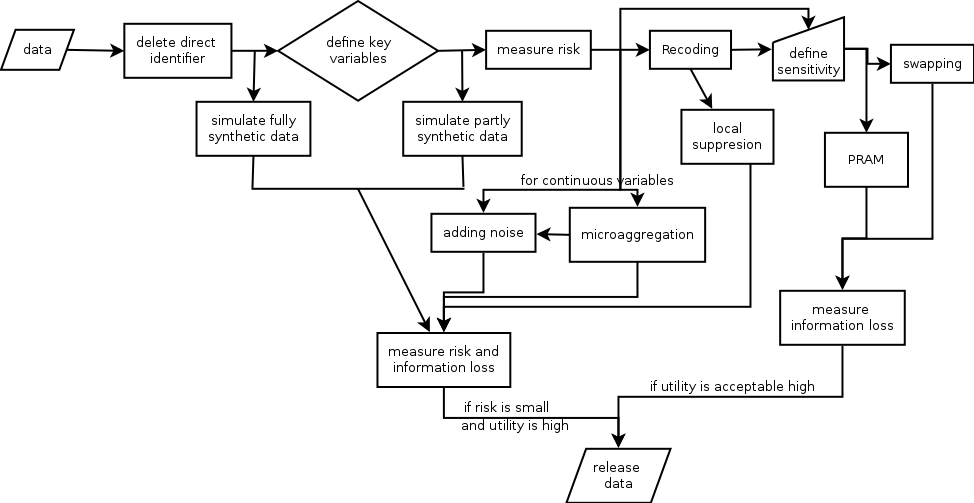
\includegraphics[width=0.95\textwidth]{ablauf}
\caption{\label{fig:ablauf}Workflow related to some of the possibilites for anonymising data using different techniques.}
\end{center}
\end{figure}

The following steps are included in Figure~\ref{fig:ablauf}.
\begin{enumerate}
\item The first step must always be to remove all direct identification variables and variables that contain direct information on 
individuals (such as name, addresses or social insurance numbers) from the data set.
\item Secondly, the key variables have to be determined. Note that this decision is subjective and 
involves discussion with subject matter specialists as well as with the interpretation of the related (national) laws 
is often necessary. Please, see Section~\ref{app} for 
practical applications to define the key variables. 
Note that for the simulation of fully synthetic data,
the choice of key variables is not necessary \citep{alfons11b}.
\item After the key variables have been selected, the disclosure risk have to be measured. 
This includes the analysis of the sample frequency counts as well as the application of 
probability methods to estimate the corresponding re-identification risk for each individual by taking
the population frequencies into account, 
see Section~\ref{method:risk_utility} for details.
\item The observations with considerable high risk may then to be perturbed. For categorical key
variables this can be done with recoding and local suppression, or with recoding and 
swapping or post randomization (pram). Note, that in principle, pram or swapping can
also be applied without recoding the key variables but the swapping rate might be defined lower
if recoding is applied first.
The decision on the method
is depended on the structure of the key variables. In general one can use recoding 
plus local suppression when
the amount of unique combinations of the key variables is low, 
and pram when the number of key variables
is large and the number of unique combinations is very high. 
For details, see Section~\ref{method:recoding}, \ref{method:pram} and 
the practical application in
Section~\ref{app}. \\
The values of continuous key variables has to be perturbed as well. 
Hereby, microaggragation is always 
a good choice (see Section~\ref{method:microagg}).
\item After the data are perurbed, the information 
loss and the disclosure risk has to be estimated.
The goal is to release a safe microdata set that has 
low risk of linking confidential information to individual respondents 
and that still has high data utility. 
If the risk is considerable low and the data utility is high, 
the anonymised data set is ready for release.
If not, the whole process has to be repeated either 
with additional perturbations (when the risk is too high) or
with actions that will increase the data utility. 
For details on issues related to 
the dependency of both the utility and the risk, see 
Section~\ref{sub:ut} and Figure~\ref{fig:rumap} that 
is discussed 
afterwards.
\end{enumerate}



\subsubsection{Simulation of Synthetic Data}

In addition, data can be also be simulated with the aim of producing 
synthetic close-to-reality data (see also Figure~\ref{fig:ablauf}).
Huge efforts are necessary to simulating synthetic data that are close-to-reality. 

Simulation of population microdata is closely related to the field of
\emph{microsimulation} \citep[e.g.,][]{clarke96}, which is a well-established
methodology within the social sciences, although the aims are quite different.
Microsimulation models attempt to reproduce the behavior of individual units
such as persons, households or firms over the course of many years for policy
\mbox{analysis} purposes. Hence they are highly complex and time-consuming.
Survey statisticians, on the other hand, need synthetic populations as a basis
for extensive simulation studies on the behavior of their statistical methods.

An alternative approach for the generation of synthetic data sets is discussed
by \citet{rubin93}. He addresses the confidentiality problem connected with the
release of publicly available microdata and proposes the generation of fully
synthetic microdata sets (all variables are generated synthetically) 
using multiple imputation. \citet{raghunathan03},
\citet{Drechsler08} and \citet{Reiter09} discuss this approach in more detail as well as
the concept of simulating only the key variables (partly synthetic data).

The generation of synthetic microdata for selected surveys  
is described by \citet{muennich03a} and
\citet{muennich03bsim}, and is further developed by
\citet{alfons11b}. 
Here, a very low number of basic categorical variables are
generated at the first stage by random draws from the actual survey data,
using the sample weights as probability weights. Additional categorical and
continuous variables are estimated with models obtained from the actual survey
data. In particular, the generation of continuous variables also involves
random draws from certain probability distributions or adding random error
terms. Since the sample weights are considered, on average \mbox{$m$-anonymity} (see the definition of
$k$-anonymity in Section~\ref{method:k_anonymity})
is provided, where $m$ denotes the smallest sampling weight. The disclosure
risk is thereby very low, because $m$ is usually high for household surveys 
\citep[for details, see, ][]{Templ10riskPop}.
Even if re-identification were successful, the corresponding observations
consist of synthetically generated values, thus rendering such a
re-identification useless.

The drawback to simulate synthetic data is that it is highly ressource-intensive from highly 
specialised researchers and
that researchers and users often feel not comfortable when they should deal with synthetic and
not real data. Because of both disadvantages, these methods are not further discussed, but we
mention the \texttt{simPopulation} \citep{simPopulation} \R -package that can be used to create synthetic data. 
We also note that the Structural Earnings Data that are used in this guidelines are created with
this package. For the methods used, we refer to \cite{alfons11b}.


\subsubsection{Remote Access and Remote Execution}

\emph{Remote access} facilities provide a flexible way to limit disclosure,
i.e., simulations with disclosive population data are performed on the data
holders' server using a secure connection, but the data itself cannot be
downloaded. However, this approach is not applicable in most countries due to
legal restrictions. With \emph{remote execution}, on the other hand, it is possible
to carry out simulations without having direct access to the data, i.e., the
user sends the code to the data holders, who apply it to the disclosive data.
Confidential results are then returned to the user. This is not a preferable
approach, though, since no model should be applied without any possibility to
explore the raw data in detail first. In addition, such a procedure can be
highly time-consuming for the data holders. Therefore, often close-to-reality synthetic data
are produced so that the users of the data can fit their models on that synthetic data first, but
for final computations, the developed code is run by the data holders stuff on the disclosive 
original data.


%This means that the estimates on anonymized data should not differ much from the original estimates.
%This means that results user perform on the protected microdata set do not differ significantly
% which results they would have obtained if the analysis was done on original data. \\


\subsection{Risk Versus Data Utility}

As mentioned before, the goal is to release a safe microdata set that has 
low risk of linking confidential information to individual respondents 
and that still has high data utility.

Figure~\ref{fig:rumap} shows a typical situation. Here, data (the SES data in Section~\ref{data:ses}) 
have been perturbed by using one specific method with different parameter values, going from 10 
(small perturbation) to 100 (perturbation is ten times higher). 
By using 100, the disclosure risk is low (since the data are heavily perturbed), but the information
loss is very high, i.e. the data utiltiy is low. Having a low perturbation, the risk and the 
data utility is high.
In any case, best is to have a method that gives you low risk and high data utility, that is the region in 
the lower left area of the figure. 


\begin{figure}[ht!]
\begin{center}
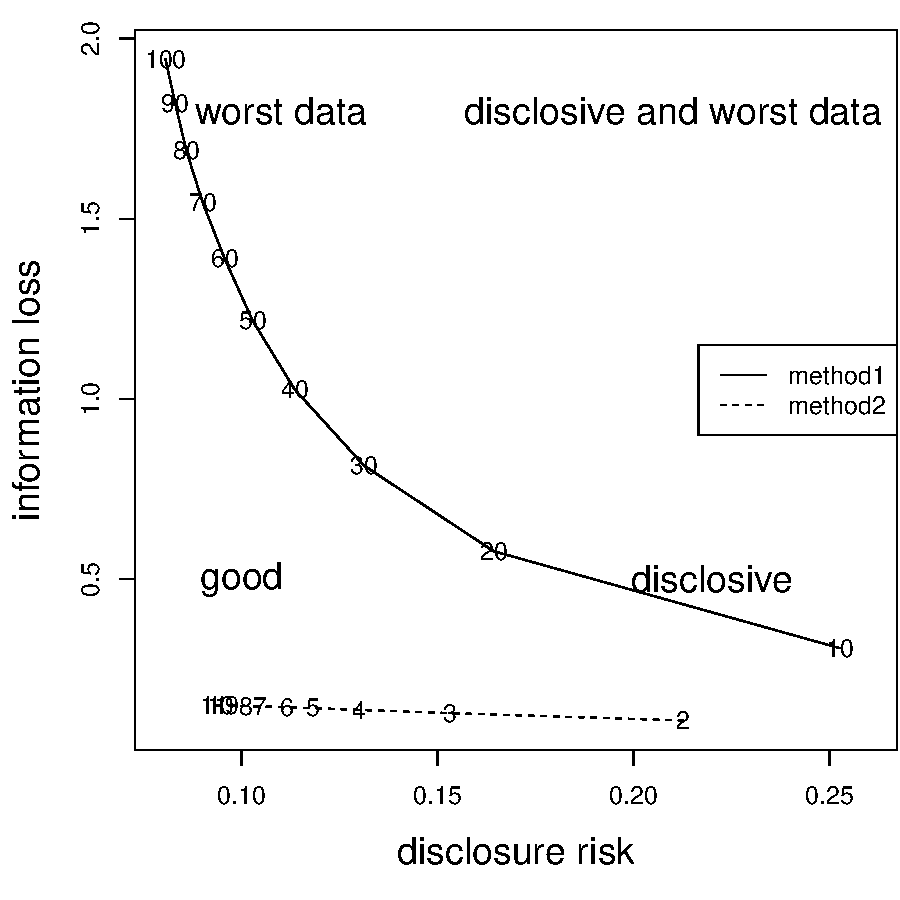
\includegraphics{guidelines-001}
\caption{\label{fig:rumap}Risk versus information loss obtained for one specific perturbation method applied on the
SES data.}
\end{center}
\end{figure}

This is not always possible and therefore the data anonymisation specialist have to make some 
decisions:
\begin{enumerate}
\item What is the legal situation regarding data privacy?
\item How sensitive is the information of the data and who will get the anonymised data file?
\item Which method is suitable for which purpose?
\end{enumerate}

\begin{description}
\item[ad 1)] Laws on privacy varying between countries. Some countries have quite restricitive laws
on data privacy, some not. Laws in one country are often different for different kind of data (business
statistics, labour force statistics, social statistics, mediacal data, etc.).
\item[ad 2)] Usually, laws consider two different kind of data users: users form universities and other 
research organisations or general users - the public. In the first case, often special contracts are signed
between the data users and the data holders. Usually, these contracts explicitely forbits the use of the data
outside a reasearch project and with the condition to save the data on a save place. 
For these kind of users, the anonymised data are called \textit{scientific use file}, whereas data
for the public are typically named \textit{public use file}. Of course, the disclosure risk of 
a public use file should be very low, and lower as for scientific use files, whereas for scientific use
files the data utility is typically higher than for public use files. \\
Another aspect is how sensitive is the information. Data on medical treatment of people might be more
sensitiv than turnover and number of employees from establishments. If the data include very sensitive
information, the data should also be protected more than data having low benefits by dislosure the
information.
\item[ad 3)] The application of some specific methods result in low disclosure risk and 
large information loss, other methods may provide data with reasonable high disclosure risk. Other methods, like
swapping or post randomisation, may provide high or low dislosure risk and data utility, depending
on the parameter choice. However, defining a swapping rate might be fixed by a data lawyer, because
the definition of disclosure risk when swapping values from, for example, every 7th observation can hereby
only be fixed by an expertise in data privacy laws and might be heavly depend on the data, on
national laws on privacy and the target user group. 
\end{description}



\subsection{The sdcMicro Package}

For each method explained we additionally show it's usage in software for both, 
via command line and
via point and click interface. 
Therefore, a small introduction to the package is given before 
the methods are explained. \\

In the last years, the statistical software environment \texttt{R} \citep{RDev}
(for short: \texttt{R}) gets more and more popular. Nowadays \texttt{R} has
more users than any other statistical software\footnote{See, for
example, \href{http://www.tiobe.com/index.php/content/paperinfo/tpci/index.html}{http://www.tiobe.com/index.php/content/paperinfo/tpci/index.html},
where \texttt{R} entered the top 20 of all programming software in January
2012. \texttt{SAS} is ranked on place 32.}, and \texttt{R} has got the standard
statistical software for data analysis and graphics. For statisticians it
has become the major programming language in its field. \\

The first version, version 1.0.0 of the \sdcMicro \ package was realeased in 2007 on the 
comprehensive \R \ archive
network (CRAN, \href{http://cran.r-project.org}{http://cran.r-project.org}). The current release, version 3.0.0, is a huge step forward.
Almost all methods have been written in \texttt{C} or do call \texttt{C++} code, so the performace
 in terms of computational speed is fine.
For the latter one, the International Household Survey Network (IHSN) provided code for that, which
is now integrated in \sdcMicro.
  
Integrating IHSN \texttt{C++} code into \texttt{R} have several benefits, 
some of which are listed below:
\begin{itemize}
  \item code written by IHSN can be used within a free and open-source 
  statistical software environment.
  \item The methods are provided within the most popular statistical software
  \item The integration of \texttt{C++} code allows fast computations in
  \texttt{R}.
  \item \texttt{sdcMicro} is a collection of microdata protection methods and
  thereby easily called.
\end{itemize}
  
After installing and starting \R , the index of methods that are available  
in the package \sdcMicro \ can be called by using the \lstinline{help} function as shown in 
Listing~\ref{listinghelp}. The package description shows a summary information about the 
package, see also Listing~\ref{listinghelpPa}.
\begin{lstlisting}[frame=single, label={listinghelpPa}, caption={Accessing the index file to list the available methods in \sdcMicro.}] 
packageDescription("sdcMicro") 
\end{lstlisting}

\begin{Schunk}
\begin{Soutput}
Package: sdcMicro
Type: Package
Title: Statistical Disclosure Control methods for the generation of
        public- and scientific-use files.
Version: 3.0.0
Date: 2012-01-30
Author: Matthias Templ, Alexander Kowarik, Bernhard Meindl
Maintainer: Matthias Templ <matthias.templ@gmail.com>
Description: Data from statistical agencies and other institutions are
        mostly confidential. This package can be used for the
        generation of anonymized (micro)data, i.e. for the generation
        of public- and scientific-use files. The package includes also
        a graphical user interface.
Depends: R (>= 2.10), robustbase, Rcpp, car, cluster, MASS, e1071,tcltk
Imports: car, robustbase, cluster, MASS, e1071, Rcpp
License: GPL-2
Packaged: 2012-01-27 16:46:04 UTC; alex
Repository: CRAN
Date/Publication: 2012-01-28 09:12:58
Built: R 2.15.0; universal-apple-darwin9.8.0; 2012-02-14 23:39:28 UTC;
        unix

-- File: /Library/Frameworks/R.framework/Versions/2.15/Resources/library/sdcMicro/Meta/package.rds 
\end{Soutput}
\end{Schunk}

%To look for the index of available methods one can type \lstinline{help(package=sdcMicro)} into \R .

One should also note that for each of the methods that has been implemented 
in \sdcMicro, a help file is available 
that not only describes all possible parameters that 
can be changed but that also features a simple, 
working example that can directly be copied into \R. The help files for a given function can be accessed by 
calling an \R-function with a \texttt{?} directly before the function name. An example is given in 
Listing~\ref{listinghelp}. 

\begin{lstlisting}[frame=single, label={listinghelp}, caption={Accessing the index of methods and the help file for function 'microaggregation' of \sdcMicro.}] 
help(package=sdcMicro)   ## index of methods
?microaggregation        ## same as help("microaggregation")
\end{lstlisting}

\sdcMicro~also features a so called vignette - a 
manual that is available in pdf-format. Such vignettes give a good overview of the capabilities 
of the software package. The vignettes contained in \R \ package \sdcMicro \ can 
be opened using the code listed in Lising~\ref{listing:vignette}. 
\textcolor{red}{
The first vignette contains a earlier report on 
\sdcMicro . The second one represents always the newest 
version of these guidelines. In the third vignette some information
about the integration of the IHSN \proglang{C++} code in \sdcMicro \ and testing of 
methods in terms of computational speed is integrated.
The latter two vignettes are included in \sdcMicro \ from version 3.1.2 onwards.}

\begin{lstlisting}[frame=single, label=listing:vignette, caption={Accessing the package vignettes of \sdcMicro.}] 
vignette("sdcMicroPaper")
vignette("sdcMicroGuideSDC")
vignette("sdcMicroTesting")
\end{lstlisting}


\subsection{The Point and Click Graphical User Interface of \texttt{sdcMicro}}

Almost all calculations can also be done using the graphical user interface (GUI) 
of \texttt{sdcMicro} - available at CRAN as the \sdcMicroGUI \ \R -package 
\citep{Templ09tdp,sdcMicroGUI}. 
The development of the new version of this GUI was funded by Google and by IHSN. 

This GUI 
serves as an easy-to-handle tool for users who want to use the \texttt{sdcMicro}
package for statistical disclosure control but are not
familiar with the native  \R \ command line interface.  
In addition to that,
interactions between objects that result from the anonymization process
are provided within this GUI. This allows an automated recalculation and
display of frequency counts, individual risk, information loss
and data utility after each anonymization step. Furthermore, the code of every
anonymization step carried out within the GUI is saved in a script, which can
easily be modified and re-used. Therefore, the GUI also allows reproducibility 
of any result.

The GUI can be installed within \R \ and called by
\begin{lstlisting}[numbers=none,captionpos=b, caption={The graphical user interface of sdcMicro.}, label=listing:gui]
install.packages("sdcMicroGUI")
library(sdcMicroGUI)
\end{lstlisting}


The GUI provides full
functionality of the main functions of \texttt{sdcMicro} and offers some more
features to the users, for example:
\begin{itemize}
  	\item comprehensive overview of the main functions and their output
	\item facilities to rename and regroup categories and to change values of a
	variable
	\item automated recalculation of frequencies and individual risk after each
	step 
	\item display of the output of the frequency and risk
	estimation interactively within the GUI 
	\item recording of the code and the selected values after each step
	\item possibility to save/load/edit a script for later re-use (reprocuible results!)
	\item (\R \ specific) no need to manually re-assign computed data to a data frame
	\item simplified load / save data option
\end{itemize}

For the basic description of the GUI, please have a look at the publication,
 which is available online for free, 
 see \cite{Templ09tdp}. Note, that the current version of the GUI includes more methods and
 the interaction with the data is revisited.

\begin{figure}[ht]
\begin{center}
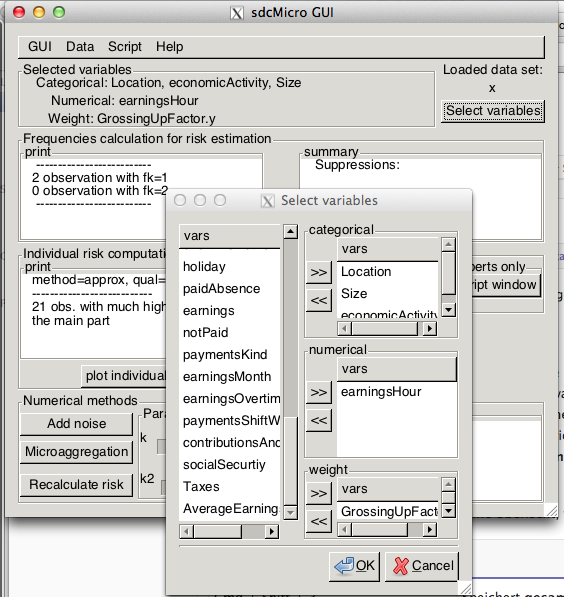
\includegraphics{gui1}
\caption{\label{fig:gui1}\textcolor{red}{NEUER SCREENSCHOT! The variable selection menu of the GUI. 
Here, some variables for the SES data are selected.}}
\end{center}
\end{figure}

Figure~\ref{fig:gui1} shows a screenshot of the GUI and it's variable selection menu. 



%\section{Methods to Proctect Microdata}
%
%We now start to introduce the important concepts of microdata anonymization. Further screenshots
%are shown in the next sections.


\section{Measuring disclosure risk}\label{method:risk_utility}
Measuring risk in an microdata set is of course of great concern 
when having to decide on wheter a 
microdata set is safe to be released. 
To be able to assess the disclosure risk it is required to make realistic assumptions on the information data users might have at hand to match against 
the microdata set. This assumptions are called 'disclosure risk scenarios'. Based on a disclosure 
risk scenario one must define a set of identifying variables (key variables) that can 
be used as input for the risk evaluation procedure. \\

Typically risk evaluation is based on the concept of ''rareness/uniqueness'' in the sample and/or in the 
population. The interest is on units/individuals/observations that possess rare combinations of key variables.
Those can be assumed to be identified easier and thus have higher risk. It is possible 
to cross tabulate all identifying variables and have a look at its cast. 
Patterns\footnote{a pattern is defined as a specific combination of values of all key variables} 
with only very few individuals are in this sense considered risky. It is also by definition that 
all units with the same values in the key variables have the same risk-value. \\


\subsection{Frequencies Counts}\label{method:Freq} 

Let us define the frequency counts also in a mathematical notation. 
Consider a random sample of size $n$ drawn from a finite population of size $N$. Let
$\pi_{j}, j = 1, \ldots, N$ be the (first order) 
\index{SDC!microdata!inclusion probability} 
inclusion probabilities, i.e. the
probability that the element $u_j$ of a population of the size $N$ is chosen 
in a sample of the size $n$. 
%Imagine that the re-identification of 
%statistical units could be performed by using external samples or registers 
%with equal variables, called 
%\index{SDC!microdata!categorical key variables} 
%(categorical) \textit{key variables}.

All possible combinations of categories in the key variables 
$X_1, \ldots, X_m$ can be calculated by cross tabulation of these categorical
variables. Let $f_i, i=1,\ldots,n$ be the 
\index{SDC!microdata!frequency counts} 
frequency counts obtained by cross
tabulation and let $F_i$ be the frequency counts of
the population which belong to the same category. If $f_i = 1$ applies 
the corresponding observation is \index{SDC!microdata!uniqueness} unique in the
sample. If $F_i = 1$ applies then the observation is unique in the population.
Note that $F_i$ is usually unknown since in statistics usually information
on samples is collected and only few information about the population is
known from registers and/or external sources - we will outline how to deal with
population frequency counts in Section~\ref{method:indivRisk} but show the basic
estimation now in the example in Listing~\ref{listingFreq}.
Here, a small example data set is loaded and the basic  
function for calculating sample frequencies  - \lstinline{freqCalc()} - is applied.
One can easily see, that observation 1 and 8 are equal and the sample frequency count is two.
The estimated population frequencies are obtained by 
summing up the sample weights for equal observations.
Here, the values of observation 1 and
8 are equal in the underlying key variables, for example. Thus the sample frequency 
counts are $f_1=2$ and
$f_8=2$. The frequency in the population $\hat{F}_1$ and $\hat{F}_8$ can
be estimated with the sum of their sampling weights, $w_1$ and $w_8$, which
equals to 110. Hence, two observations with the pattern $(1,2,5,1)$ exist in the
sample and 110 observations with these entities can be expected to exist in the
population.


\begin{lstlisting}[captionpos=b, caption={Example for sample and estimated population frequency counts.}, label=listingFreq]
require(sdcMicro)
data(francdat)
x <- francdat[,c(2,4,5,6,8)]
ff <- freqCalc(x, keyVars=1:4, w=5) 
print(cbind(x, ff$fk, ff$Fk))
  Key1 Key2 Key3 Key4     w ff$fk ff$Fk
1    1    2    5    1  18.0     2 110.0
2    1    2    1    1  45.5     2  84.5
3    1    2    1    1  39.0     2  84.5
4    3    3    1    5  17.0     1  17.0
5    4    3    1    4 541.0     1 541.0
6    4    3    1    1   8.0     1   8.0
7    6    2    1    5   5.0     1   5.0
8    1    2    5    1  92.0     2 110.0
\end{lstlisting}

\lstinline{freqCalc()} includes basically three parameters which could be displayed in \R \ 
either using
\begin{lstlisting}[frame=single, label=code:sdcMicro6,
caption={Displaying the arguments of function {\tt freqCalc()}.}]
args(freqCalc) 
  function (x, keyVars = 1:3, w = 4, ...)
\end{lstlisting}
or typing \texttt{?freqCalc} which displays the whole help file.
\texttt{x} is an object of class data.frame or matrix, \texttt{keyVars} is a
vector specifying the column index of the key variables and \texttt{w}
defines the column index of the weight variable. The resulting output of the
function are the frequency counts of the sample and the estimated frequency
counts of the population.
Note that by using the point and click interface of \sdcMicro, 
the \sdcMicroGUI, the frequencies are calculated automatically at every step 
of the anonymisation process.

\subsection{The $k$-Anonymity Concept}
\label{method:k_anonymity}

Based on a set of key variables a desired characteristic of a protected microdata set might be to 
achieve the concept of $k$-anonymity \citep{Samarati98,Sweeney02}. 
This means that each possible combination of the values of the key variables 
features at least $k$ units in the microdata, meaning that 
all $f_i \geq 3 \ , i=1,...,n$ \ .
A typical value is $k=3$. \\

$k$-anonymity is typically achieved by recoding categorical key variables 
(see Section~\ref{method:recoding}) and by 
additionally suppressing specific values in the key variables of individual units 
(Section~\ref{method:localsupp}).



 
%and local suppression (function
%\lstinline{localSuppression()}) can be applied, see Section~\ref{app} for practical applications. 
For local suppression, function \lstinline{localSuppression()} to accomplish $k$-anonymity can be used. Hereby, 
a heuristic algorithm is called to suppress as few values as possible. 
Provided as a function argument, it is possible to 
specify a desired ordering of key variables which the algorithm takes into account 
when performing the local suppression. 
One could even specify key variables that are considered of such importance that almost 
no values in these variables are suppressed. All functions can also be used by point and click in the \sdcMicroGUI .\\

\subsection{$l$-Diversity}

An extension of $k$-anonymity is $l$-diversity \citep{Machanava07}. 
%This method gives  stronger privacy guarantees but $k$-anonymity is 
%much easier to apply.
Consider for one group of observations with the same pattern in the key variables and let the
group fulfil $k$-anonymity. A possible data intruder can therefore not identify an individual 
in this group. However, if all observations have the same entries in a sensitive variable (such as
\textit{cancer} in the variable \textit{medical diagnosis}) then the attack is successful anyway. For example,
with the knowledge that one individual is in the group - say the individual's name is Carl Carlson - 
then you know that Carl has cancer with certainty  if all members in that group have cancer. 
The distribution of the target sensitive variable is refered to as $l$-diversity.

\begin{lstlisting}[captionpos=b, caption={k-anonymity and l-diversity.}, label=listingFreq2]
x <- data.frame(key1=c(1,1,1,1,2,2), key2=c(1,1,1,2,2,2), sens1=c(50,50,42,42,62,62))
ff <- freqCalc(x, keyVars=1:2, w=NULL)
div <- measure_risk(x, keyVars=c("key1","key2"), ldiv_index="sens1")
cbind(x, ff$fk, div$ldiv[,1])
  key1 key2 sens1 ff$fk sens1_Distinct_Ldiversity 
1    1    1    50     3                         2               
2    1    1    50     3                         2               
3    1    1    42     3                         2                
4    1    2    42     1                         1                
5    2    2    62     2                         1               
6    2    2    62     2                         1                
\end{lstlisting}

In Listing~\ref{listingFreq2} we consider a small example data set that should highlight the
calculations related to get the   
$l$-diversity. It also points out the (slight) difference to $k$-anonymity. 
In the first two columns the categorical 
key variables are present. The third column of \texttt{x} defines a variable containing 
sensitive information. The sample frequency counts have been calculated and present in the fourth 
column. They are equal 3 for the first three observations, the fourth observation is unique and for the
last two observations, the frequency counts are 2. Only observation four violates $2$-anonymity. 
When having a closer look at the first three observations
we see that only two different values are present in the sensitive variable, 
so the $l$-(distinct)-diversity is
just 2. For the last two observations, $k$-anonymity is achieved but still the intruder knows the exact information of the sensitive variable
. However, the $l$-diversity is 1 indicating that the sensitive information can be disclosed, since 
all values are equal in 
the sensitive variable ($=62$). 

The difference in values in the sensitive variable can be measured in different ways - here we presented only
the distinct diversity that measures how many different observations are present in a group. Other methods
are implemented for $l$-diversity in \sdcMicro \ (entropy, recursive, multi-recursive) as well, see the help
manual of the package for further information.


\subsection{Considering Sample Frequencies on Subsets: SUDA}\label{method:suda}

SUDA 
 (\textbf{S}pecial \textbf{U}niques \textbf{D}etection \textbf{A}lgorithm) 
estimates a disclosure risk for each individual. 
 SUDA2 \citep[see, e.g.,][]{manning08} is a recursive algorithm for finding
Minimal Sample Uniques. The algorithm generates all possible
variable subsets of defined categorical key variables 
and scans them for unique patterns in the subsets of variables. The risk of an observation is then dependend on two 
aspects.
\begin{itemize}
\item[(a)] The lower the
amount of variables needed to receive uniqueness, the higher the risk (and the higher the 
\textit{suda score}) of the
corresponding observation. 
\item[(b)] The larger the number of
minimal sample uniquenes contained within an observation, the higher the risk of the observation.
\end{itemize}

(a) is calculated for each observation $i$ by $l_i = \prod_{k=MSUmin_i}^{m-1} (m-k) \quad , i=1,...,n$, 
for $m$ the \textit{depth} (the maximum size of variable subsets of the key variables),  
$MSUmin_i$ the number of minimal uniques of observation $i$ and $n$ the 
number of observations of the data set. 
Since each observation is treated independently, the $l_i$ that belongs to one pattern are summed up 
to result in a common suda score for each of the observation belonging to this pattern 
(this summation is the contriubtion of (b)).

To result in the final SUDA score, the suda score are normalized due division 
by $p!$, with $p$ being the number of key variables.

To receive the so called DIS score, 
loosely speaking, an iterative algorithm based on sampling of the data and matching of subsets of the sampled data 
with the orginal data is applied, 
whereas the probilities of correct matches given unique matches are
calculated. In fact, it is out of scope to exactly describe the algorithm but we refer to
\cite{Elliot00} for details. The DIS suda score is
then calculated from the suda and the DIS scores
(in \sdcMicro \ \texttt{disScore}).

 Note that this method does also not consider population frequencies in general but consider 
 sample frequencies on subsets. The dis sudo scores somehow approximately consider 
 based on the sample information - population uniqueness
 by simulation, but - to our knowledge - in generally it do not consider 
 sampling weights and biased estimates may therefore result.

\begin{lstlisting}[captionpos=b, caption={Example showing how to estimate suda scores.}, label=listingsuda]
data(francdat)
x <- francdat[,c(2,4,5,6,8)]
ff <- freqCalc(x, keyVars=1:4, w=5)
s <- suda2(francdat, variables=1:4)
cbind(x[,1:4], ff$fk, s$score, s$disScore)
  Key1 Key2 Key3 Key4 ff$fk s$score  s$disScore
1    1    2    5    1     2    0.00 0.000000000
2    1    2    1    1     2    0.00 0.000000000
3    1    2    1    1     2    0.00 0.000000000
4    3    3    1    5     1    3.50 0.016380722
5    4    3    1    4     1    0.00 0.000000000
6    4    3    1    1     1    0.00 0.000000000
7    6    2    1    5     1    1.75 0.007196697
8    1    2    5    1     2    0.00 0.000000000
\end{lstlisting}

In Listing~\ref{listingsuda} again the example data set already 
used in Section~\ref{method:Freq} is used
and the frequency counts but also the suda and dis suda scores are calculated. 
The suda scores are largest for observation 4 since also subsets of observation four are unique, while
for observation five and six, not any subset is unique.


Suda, in fact suda2 \citep[SUDA2,][]{manning08}, is  
 implemented in \sdcMicro~ 
  (function \lstinline{suda2()}) based on \texttt{C++} code 
  from the IHSN. %\textit{Organization of Economic Co-Operation and Development} (OECD). 
 
Additional output, like the contribution percentage of each variable to the score, 
is also valued as function output.
The contribution to the suda 
score is simple calculated by looking how often a category of a key variable contributes to the score.
 
 


\subsection{Considering Population Frequencies - The Individual Risk Approach}\label{method:indivRisk}


To define if an individual unit is at risk, typically a threshold approach is used.
 If the invidual risk of reidentification for an individual is above a certain threshold value, 
 the unit is said to be at risk. To calculate the individual risks it is neccessary 
 to estimate the frequency 
 of a given key in the population. 
 In the previous section, Section~\ref{method:Freq}, the population frequencies are already 
estimated. However, one can show that these estimates almost always overestimate small 
population frequency counts \citep[details can be found in]{templ11book} and should not be used
to estimate the disclosure risk.

A better approach is to use so called superpopulation models  
 (the population frequency counts are modelled by 
 a certain distribution). 
 The whole estimation procedure of sample counts given the population counts can be modeled, 
 for example, by using a 
 Negative Binomial distribution \citep[see, e.g.,][]{Rinott06} and is implemented 
 in \sdcMicro~in function \lstinline{measure_risk()} %\lstinline{indivRisk()} 
 \citep[for details, see][]{templ11book}, and, of course, it can be called within the 
 point and click GUI. 

In Listing~\ref{listingIndiv} all concepts are applied once again - the frequency count estimation on 
sample and population level (sum of the weights for each group), the $l$-diversity, 
the suda algorithm and the individual risk estimation. One can see that the individual risk is low 
for observation five, for example, since the sampling weight is quite high and therefore one may expect 
no population uniqueness. On the other hand, the individual risk is especially high for sample uniqueness in combination with
small sampling weights, i.e. the inclusion probability of each individual is respected when estimating the
individual risk.

\begin{lstlisting}[captionpos=b, caption={Estimating the risk.}, label=listingIndiv]
data(francdat)
x <- francdat[,c(2,4,5,6,1,8)]
ff <- freqCalc(x, keyVars=1:4, w=6) # frequencies
div <- measure_risk(x, keyVars=1:4, ldiv_index=5,w=6)
s <- suda2(francdat, variables=1:4) # suda
cbind(x, freqS=ff$fk, freqP=ff$Fk, ldiv=div$ldiv[,1], suda=s$score, indivR=round(indivRisk(ff)$rk,3))
  Key1 Key2 Key3 Key4 Num1     w freqS freqP ldiv suda indivR
1    1    2    5    1 0.30  18.0     2 110.0    0 0.00  0.017
2    1    2    1    1 0.12  45.5     2  84.5    0 0.00  0.022
3    1    2    1    1 0.18  39.0     2  84.5    0 0.00  0.022
4    3    3    1    5 1.90  17.0     1  17.0    0 3.50  0.177
5    4    3    1    4 1.00 541.0     1 541.0    0 0.00  0.011
6    4    3    1    1 1.00   8.0     1   8.0    0 0.00  0.297
7    6    2    1    5 0.10   5.0     1   5.0    0 1.75  0.402
8    1    2    5    1 0.15  92.0     2 110.0    0 0.00  0.017
\end{lstlisting}



\subsection{Measuring the Global Risk}

Although the individiual risk have to be respected since a data intruder 
should not be able to identify individuals, 
often also a measure of the global risk is estimated in order to have one number 
that expresses the 
risk of the whole data set.


\subsubsection{Measuring the Global Risk Based on the Individual Risks}

The first approach is to determine a threshold for the individiual risk and to calculate 
the percentage of individuals that have larger individual risk than this threshold.
The output can be seen in Listing~\ref{listingGR}.

\begin{lstlisting}[captionpos=b, caption={Estimating the global risk.}, label=listingGR]
data(francdat)
x <- francdat[,c(2,4,5,6,1,8)]
ff <- freqCalc(x, keyVars=1:4, w=6) # frequencies
(measure_risk(x, keyVars=1:4, w=6, max_global_risk = 0.1))
--------------------------
3 obs. with much higher risk than the main part
Expected no. of re-identifications:
 0.97 ( 12.08 %)
Threshold: 0.18 
 (for maximal global risk 0.1 )
--------------------------
\end{lstlisting}


\subsubsection{Measuring the Risk Using Log-Linear Models}

The sample frequencies, considered for each of $M$ patterns $m$, $f_m \ , m=1,...,M$ 
can be modeled by a 
Poisson distribution, and the global risk may be defined as \citep[see][]{Skinner98}
\begin{equation}
\tau_1 = \sum\limits_{m=1}^{M} \exp\left( -\frac{\mu_m (1 - \pi_m)}{\pi_m}\right)  \quad \mu_m=\pi_m \lambda_m \quad .
\end{equation}
For simplicity, the inclusion probabilities are assumed to be equal, $\pi_m=\pi \ , m=1,...,M$.
$\tau_1$ can be estimated by log-linear models including the main effects and possible interactions.
The model is
\begin{displaymath}
\log (\pi_m \lambda_m) = \log (\mu_m) = \mathbf{x}_m \mathbf{\beta} \quad .
\end{displaymath}

To estimate the $\mu_m$'s, the regression coefficients $\mathbf{\beta}$ have to be estimated, for
example by the iterative proportional fitting approach that is used  
in function \lstinline{LLmodGlobalRisk()}.



\section{Measuring data utility} \label{sub:ut}

Of couse it is also of great interest to measure the data utility of the microdata set after disclosure 
limitation methods have been applied. 

\subsection{General Applicable Methods}

Anonymized data should have the same structure of the original data 
and should allow any analysis with high precision.

To evaluate the precision, the estimation of different classical estimates like means and covariances are in focus.
Using \lstinline{dUtility()} it is possible to calculate 
several different measures on continuous scaled variables 
that are based on classical or robust distances. These estimates are computed for the original data and the 
perturbed data and they are finaly compared with the estimates on the original data. 

For evaluating the multivariate structure of perturbed data, 
comparisons based on eigenvalues and robust eigenvalues 
can be also made with function \lstinline{dUtility()}. 



\subsection{Specific Tools}


In practice it is not possible to create an anonymized file 
 that have exactly the same structure as the 
orginal file in every sense. However, the difference between estimations with anonymized and 
original data of the \textbf{most important statistics} should be very small or even zero.
This approach is therefore to measure the data utility based on benchmarking indicators 
\citep{ichim10,templ11ses} and is a more serious approach than applying general tools. \\

The first step in assessing quality is to decide on a set of benchmarking
indicators. In order to do so, one has to evaluate 
what the users of the underlying data are analysing and report on the most 
important estimates. These estimators are often called 
\textit{benchmarking indicators} \citep[see, e.g.,][]{templ11unece,templ11ses}.
Special emphasis should be put on benchmarking indicators with
respect to the most important variables but also to the most sensible variables
within the micro data set. \\

The general procedure is quite simple and can be described in the following
steps:
\begin{itemize}
  \item Selection of a set of benchmarking indicators
  \item Choice of a set of criteria on how to compare indicators
  \item Calculation of all benchmarking indicators on the original, unmodified
  micro data set
  \item Calculation of the benchmarking indicators on the protected
  micro data set
  \item Comparison of statistical properties such as point estimates, variances
  or overlaps in confidence intervals for each benchmarking indicator 
  \item Assessment if the data utility of the protected micro data set is good
  enough to be used by researchers
\end{itemize}

If the quality assessment in the last step of the sketched algorithm is
positive, the anonymized micro data set may be published. If the deviations of
the main indicators calculated from the original and the protected data are too
large one should restart the anonymization procedure and either modify selected
parameters or completely change the anonymization process.

Usually the evaluation is focused on the properties of numeric
variables given unmodified and modified micro data. However, it is of course
also possible to have a look at the impact of local suppression or recoding that
has been conducted to reduce individual reidentification risks. 

Another possibility to evaluate the data utility of numerical variables is to
define a model that is fitted on the original, unmodified microdata. The main
idea is to predict important, sensitive variables using this model both for the
original and the protected micro data set in a first step. In a second step,
statistical properties of the model results, such as the differences in
point-estimates or variances are compared for the predictions given original and
modified micro data, are compared and the resulting quality is assessed. If the
deviations are small enough one may go on to publish the safe and protected
micro data set. Otherweise adjustments in the protection procedure need to be
done.

Also, it is interesting to evaluate the set of benchmarking indicators not only
for the entire data set but also for some domains. In this case the data set is
partitioned into a set of $h$ groups. The evaulation of benchmarking indicators
is then performed for each of the $h$ groups and results are evaluated by
looking at differences between indicators for original and modified data in each
group.




In this report, Appendix~\ref{sec:ind} gives a detailed description on the benchmarking indicators 
for the data used in this report. For the detailed application to real data and discussion theirein, 
see Section~\ref{sec:utility2}.


%%%%%%%%%%%%%%%%%%%%%%%%%%%%%%%%%%%%%%%%%%%%%%%%%%%%%%%%%%%%%%%%%%%%

\subsection{Recoding}\label{method:recoding}
Recoding is a non-perturbative method that can be applied to both categorical and continous variables. If global recoding is applied to a categorical variable the main idea is to combine several categories into a new, less informative category. When the method is applied to a continous variable it means to discretize the variable. The main idea is in both cases to reduce the total number of possible outcomes of the variable under consideration. Typically, recoding is applied to categorical variables where it is possible to reduce the number of categories with a small number of observations (extreme categories). \\

A special case of global recoding is 'top and bottom coding' which can be applied to ordinal and categorical variables. The main idea for this approach is to combine all values above (top-coding) and/or below (bottom-coding) pre-specified threshold values into a new category. \\

Function \lstinline{globalRecode()} can be applied in \sdcMicro~to perform global recoding and also top/bottom coding. 
The help file with some examples is accessible using \lstinline{?globalRecode}. Note, that a more user-friendly version of global recoding 
can be applied using the graphical user interface of \sdcMicro .


\subsection{Local Suppression}\label{method:localsupp}
Local suppression is a non-perturbative method that is typically applied to categorical variables. 
The key-idea is to suppress certain values of one or more variables. 
Typically the input variables are part of the defined set of 
key variables that are used for risk-calculations as it was described in \ref{method:risk_utility}. 
Individual values are suppressed in a way that the set of variables aggreeing on a specific combination of values of 
key variables are increased. Local suppression is often used to achieve the goal of $k$-Anonymity as described in 
Section~\ref{method:k_anonymity}. \\

Using function \lstinline{localSupp()} of \sdcMicro~it is possible to
 suppress the values of a key-variable for all those individual units for which the calculated individual 
risk of reidentification given a disclosure risk scenario is above a threshold. 
This is somehow a manual method.

For automatically suppress a minimum amount of values in the key variables to achieve $k$-anonymity, function
\lstinline{localSuppression()} can be used.


\begin{lstlisting}[captionpos=b, caption={Local Suppression to achieve k-anonymity.}, label=listingGR]
data(francdat)
## Local Suppression            
localS <- localSuppression(francdat, keyVar=c(4,5,6))
localS
 -----------------------
[1] "Total Suppressions in the key variables -2"
[1] "Number of suppressions in the key variables "

 0 0 2 
 ------------
[1] "2-anonymity == TRUE"
 -----------------------
\end{lstlisting}

Note that the importance of variables can be specified as a parameter in function
\lstinline{localSuppression()}, aiming that some variables might be
prefered for suppression while in some variables should only a minimum of
suppression been done to achieve $k$-anonymity for all key variables.






\subsection{Post-Randomization}\label{method:pram}
Post-Randomization (equivalently referred to as PRAM) \citep{Gouweleeuw98} is a perturbative, 
probabilistic method that can be applied to categorical variables. 
The key idea is that the values of a categorical variable 
in the original microdata file are changed into other categories with resprect to a pre-defined transition probabilities.
%to a pre-defined transition process. 
This process is usually modeled using a known transition matrix 
in which for each possible category of a categorical variable a probabilty for each transition to another category
 is specified. %This distribution determines probabilities that the original data value is changed to any other score. \\
A simplified example would be to have a varibles with three categories/classes, A1, A2 and A3. 
The transition of 
a value from category A1 to category is, for example, fixed at $0.15$, meaning with
 probability $p_1=0.85$ a value is not changed from A1 to A2.
A value changed to A2 is fixed with probability $p_2=0.1$ and 
changed to A3 with $p_3=0.05$. 
Also probabilites to change values from class A2 to the other classes and for A3, respectively, have to be fixed.
This is stored in 
a matrix of such transition probability which is the main input to function \lstinline{pram()} in \texttt{sdcMicro}.
This above mentioned example is used in Listing~\ref{listingPram} whereas the default parameters of \lstinline{pram()} are used.
One can see that one value changed the category.
\begin{lstlisting}[captionpos=b, caption={Example for pram.}, label=listingPram]
set.seed(1234)
A <- as.factor(rep(c("A1","A2","A3"), each=5))
A
 [1] A1 A1 A1 A1 A1 A2 A2 A2 A2 A2 A3 A3 A3 A3 A3
Levels: A1 A2 A3
Apramed <- pram(A)
Apramed
...
 Parameters for PRAM: 
 alpha =  0.5
 minimum diagonal element =  0.8 
 
summary(Apramed)
 ----------------------
 original frequencies:
A1 A2 A3 
 5  5  5 
 ----------------------
 frequencies after perturbation:
A1 A2 A3 
 6  4  5 
 ----------------------
 transitions:
  transition Frequency
1    1 --> 1         5
2    2 --> 1         1
3    2 --> 2         4
4    3 --> 3         5
\end{lstlisting}


PRAM is applied to each observation independently and the procedure is random, meaning that 
without setting a seed, different solutions are obtained for every call of \lstinline{pram()} or \lstinline{pram_strat()}.% and can be applied to one or more categorical variables. 
 One should note that the method is quite flexible since the transition matrix can be specified freely as a function parameter. \\

Two implementations are available in \sdcMicro : \lstinline{pram()} and \lstinline{pram_strat()}, 
the corresponding help files can be accessed with \lstinline{?pram} or \lstinline{?pram_strat}. 
With the latter one includes a stratified version of pram.


\subsection{Microaggregation}\label{method:microagg}
Microaggregation is a perturbative method that is typically applied to continous variables. 
The main idea is that records are partitioned into groups. Within each group values of each variable are 
aggregated (typically the mean is used). The individual values of the records for each variables are finally  
replaced by the group aggregation, see e.g. Listing~\ref{listingMicroaggregation} where always two values that are most similar
are replaced by their columnwise means.
\begin{lstlisting}[captionpos=b, caption={Example for microaggregation.}, label=listingMicroaggregation]
data(francdat)
x <- francdat[,c(1,3,7)]
m <- microaggregation(x, aggr=2)
mx <- m$mx
colnames(mx) <- c("MicNum1","MicNum2","MicNum2")
cbind(x, mx)
  Num1 Num2 Num3 MicNum1 MicNum2 MicNum2
1 0.30 0.40    4   0.240   0.600     6.0
2 0.12 0.22   22   0.560   0.760    17.5
3 0.18 0.80    8   0.240   0.600     6.0
4 1.90 9.00   91   1.450   5.200    52.5
5 1.00 1.30   13   0.560   0.760    17.5
6 1.00 1.40   14   1.450   5.200    52.5
7 0.10 0.01    1   0.125   0.255     3.0
8 0.15 0.50    5   0.125   0.255     3.0
\end{lstlisting}

In function \lstinline{microaggregation()}
parameters for the method used, the aggregation level (how many observations are 
combined) and the statistics that is used to calculate the aggregation statistics (default $=$ arithmetic mean).\\ 

%\sdcMicro~features a set of different algorithms to specify the algorithm. It is possible to 
%form the groups using multivariate distances with classical or robust methods \citep{Templ08d}. 
%It is also possible to perform the grouping using different clustering algorithms, 
%principal component analysis or to use classical or robust projection methods.  
%The user can define the group sizes and of course specify the proximity measure. \\

All of the above settings (and many more) can be applied in \sdcMicro~using 
function \lstinline{microaggregation()}. The corresponding help file can be 
viewed with command \lstinline{?microaggregation}. A plot method is available, just type 
\lstinline{plot(m)}, where $m$ is an object of class "micro".


\subsection{Adding noise}\label{method:noise}
Adding noise is a perturbative microdata protection method that is 
typically applied to continous variables. 
The main idea is to add statistical noise to a given continous 
variable. This approach protects data against exact matching 
with external files if information on specific variables is 
available e.g. from registers.\\

While this approach sounds simple in principle, a lot of different algorithms can be used to 
add (stochastic) noise. It is possible to add uncorrelated random noise where the noise 
is typically normally distributed with the variance of the noise term is proportional to the variance 
of the original data vector. Adding uncorrelated noise preserves means but variances 
and correlation coefficients between variables are not preserved while this is respected for the correlated noise method(s). 
%It is however also possible to overlay the original data values with correlated noise \citep{Brand04}. 
For the correlated noise method \citep{Brand04} 
the noise term derived from a distribution with a covariance matrix that is proportional 
to the covariance matrix of the original microdata set. 
In the case of correlated noise addition, correlation coefficients are preserved 
and at least the covariance matrix can be consistently estimated from the perturbed data. However, the data structure may differ 
a lot if the assumption of normality is violated. Since this is virtually always the case when working with real-world data,
a robust version of the correlated noise method is included in \sdcMicro \ (more details can be found in the help file
of the package by calling \texttt{?addNoise} and in \cite{Templ08f}) that allows departures from model assumptions.\\

In \sdcMicro~several other algorithms are available that can be used to add noise to continous variables. 
For example it is possible to add noise only to outlying observations for which the assumtion 
is that such observations possess higher risk than non-outlying observations or to 
make sure that the amount of noise that should be added takes account 
the underlying sample sizes. \\

Noise can be added to variables in \sdcMicro~using function \lstinline{addNoise()}. 
The help file can be shown by typing \lstinline{?addNoise}.

Listing~\ref{listingADD} shows how this function can be applied with \sdcMicro .

\begin{lstlisting}[captionpos=b, caption={Example for adding correlated noise to continuous variables.}, label=listingADD]
a <- addNoise(x, method="correlated2")$xm
\end{lstlisting}


%%%%%%%%%%%%%%%%%%%%%%%%%%%%%%%%
%%% Description of data sets %%%
%%%%%%%%%%%%%%%%%%%%%%%%%%%%%%%%

%%%%%%%%%%%%%%%%%%%%%%%%%%%%%
%%% Practical application %%%
%%%%%%%%%%%%%%%%%%%%%%%%%%%%%
\section{Practical Application}\label{app}

% Why is protection needed? -> legal reasons?
% What are key-characteristics and use of the data
% What is the disclosure risk of the "unmodified data"
% Apply limitation techniques using software -> different methods for different users and possible data uses
% Reassess disclosure risk
% publish protected microdata


% Perturbative vs. non-perturbative methods
% Risk vs. information loss


In this section we show how to apply the concepts and methods 
introduced in Section~\ref{overview:methods} using \sdcMicro. 

\subsection{Pre-processing steps}

The first step is to start \R, install \sdcMicro~from CRAN and load the package as it is shown 
in Listing \ref{listing:install}.

\begin{lstlisting}[captionpos=b, caption={Installing and loading \sdcMicro.}, label=listing:install]
install.packages('sdcMicro')
library(sdcMicro)
\end{lstlisting}


Once the package is loaded, we can use all the functions and methods that the
package provides. For an overview the user is advised to have a look at the manual which 
can be accessed by typing \lstinline{help(package=sdcMicro)} into the \texttt{R} console. \\

The first step in creating safe microdata is of course a very accurate 
analysis of the raw data set to get an idea about key-characteristics and possible use of the data. 
Furthermore it is also neccessary to take into account legal considerations. 
Especially it is important to define which properties are required 
from a microdata set that it can be considered safe. Since legal regulations vary from 
country to country it is not possible to define general rules. These judgements have to 
be made by subject matter experts.\\

\subsection{Data sets under consideration} \label{data:descr}
In this Section we show how to apply the disclosure limitation techniques 
discussed in Section \ref{overview:methods} to two different data sets. 
It is worth mentioning that the anonymization methods applied on data that are saved in flat files.

We will now give an overview about the microdata sets under consideration and refer to Annex~\ref{annex:data} to 
a more detailed overview of the data.


\subsubsection{FIES}
The \textit{Family Income and Expenditure Survey} (FIES) from 2006 data has been 
provided by the National Statistics Office of the Philippines. 
It is a household survey to gather information on family income and expeditures and it is also been used to
measure inequality.

\subsubsection{SES}
The Structural Earnings Survey (SES) is conducted in almost all European
countries and it includes variables on earnings of employees and other variables on 
employees and employment level (e.g. region, size of the enterprise, economic activities of the enterprise, 
gender and age of the employees, \ldots).

%Details about these data sets are included in Annex~\ref{annex:data}.


\subsection{General approach}

To create safe microdata files for both the FIES and the SES data set, we will take the following approach. 
\begin{enumerate}
\item define a set of key variables and thus a disclosure risk scenario
	\item assess the disclosure risk of the unmodified data
	\item possibly perform recoding of variables 
	\item achieve $k$-anonymity within the key variables by local suppression
	\item reassess disclosure risk after local suppression
	\item protect numeric variables using suitable methods
	\item remove additional information from microdata set if it is neccessary
\end{enumerate}

In Section \ref{app:fies} and \ref{app:ses} we will now show how 
to transform a microdata set into a safe microdata file that could be published. 
It must be noted however that the purpose of this document is to create guidelines and not 
to actually create a safe microdata set.

\subsection{Application to FIES data}\label{app:fies} 

% Code in Daten/anonFies.r

The first step consists in loading the data into \R. In this case 
the microdata are already available as a \R-data file and can easily be 
loaded as shown in Listing \ref{listing:load.fies}.

\begin{lstlisting}[captionpos=b, caption={Loading microdata into \R.}, label=listing:load.fies]
data <- load('FIES06V2.RData')
\end{lstlisting}

We observe that in the data set no direct identifiers such as names or adresses
exist. Thus it is not required to remove any variables from the data set now. Looking at the data and its metadata\footnote{available in xml-file format.} we learn that the statistical units are households and the microdata set is the result of a survey. It is therefore important to take survey weights into account if we want to asses the disclosure risk. The variable holding sampling weights is called ''rfact''. \\

The next step consists of deciding on a set of key variables that attacker could use to identify households. In this case we 
arbitrarily\footnote{since we do not have any knowledge which information might be available to attackers in the Philippines 
from registers or other data sources.} choose the following variables to be key variables.
\begin{itemize}
	\item {\bf w\textunderscore regn}: region with 17 characteristics
	\item {\bf z2011\textunderscore h\textunderscore sex}: sex with 2 characteristics
	\item {\bf z2021\textunderscore h\textunderscore age}: age with 86 characteristics
	\item {\bf z2041\textunderscore h\textunderscore educ}: educational attainment with 21 characteristics
\end{itemize}

We now assess the disclosure risk given our choice of key variables. In Listing \ref{listing:freq1} it is shown how to set up the disclosure scenario. 
\begin{lstlisting}[captionpos=b, caption={Performing frequency calculations}, label=listing:freq1]
kVars <- c('w_regn','z2011_h_sex','z2021_h_age','z2041_h_educ')
keyVars <- match(kVars, colnames(dat))
weightVar <- match('rfact', colnames(dat))
(fk <- freqCalc(dat, keyVars, weightVar))
\end{lstlisting}
First the key variables are defined and its position in the dataset is 
calculated (lines 1 and 2). Since we are dealing with sample data it is also required 
to define the variable holding sample weights and to calculate its position within 
the microdata set which is done in line 3. In line 4 the actual calculation of 
frequencies at survey and population level within possible keys is performed and the results of the frequencies at
population level are printed in code listing \ref{listing:results:freq1}.

\begin{lstlisting}[numbers=none,captionpos=b, caption={Results of first frequency calculation}, label=listing:results:freq1]
4506 observation with fk=1 
3562 observation with fk=2 
\end{lstlisting}

We see that a total of 4506 keys is unique in the sample (fk=1) and additionally 3562 combinations of 
characteristics of key variables are occupied only by two units (fk=2). 
Note, that the corresponding estimates for population frequencies are stored in the object \texttt{fk}. 
They are estimated with help of the sampling weights and therefore not suitable for risk estimation \citep[for details have a look at][]{templ09diss}.
Therefore a theoretical distribution for the frequency counts of the population with respect to the frequency counts 
in the sample is usually chosen and theoretical values of this superpopulation distribution are used for 
risk estimation \citep[for details, see][]{Rinott06}.
Listing~\ref{listing:risk1} shows how 
to assess the disclosure risk of the unmodified microdata set in practice.

\begin{lstlisting}[captionpos=b, caption={Assessing disclosure risk of unmodified microdata}, label=listing:risk1]
rk <- indivRisk(fk, survey=TRUE)
plot(rk)
\end{lstlisting}
Function \lstinline{indivRisk()} is called with two parameters. 
The first input parameter is an object of class ''freqCalc'' derived by using 
function \lstinline{freqCalc()}. The second parameter survey has to be set to ''TRUE'' if one deals 
with survey data as it is the case here. Figure \ref{graph:risk1} (produced by simple calling plot() on the object \texttt{rk}, see 
Listing~\ref{listing:risk1}) shows the distribution of the risks. 

It is easy to see that some observations have high risk of disclosure, i.e. 
we observe that some units are clearly at risk to be identified with respect to
the chosen set of key variables when choosing the maximum individual risk at 5\%, for example.

%pdf("risk1.pdf", width=9, height=6)
%par(mfrow=c(1,2))
%par(oma=c(1,1,1,1))
%hist(rk$rk, col="grey", main="individual risk evaluation\nkey-vars: %region|age|sex|educ", xlab="Risk", ylab="Frequency")
%plot(ecdf(rk$rk), main="empirical distribution function\n of individual risks", %xlab="Risk", ylab="Probability")
%dev.off()

\begin{figure}
	\centering
	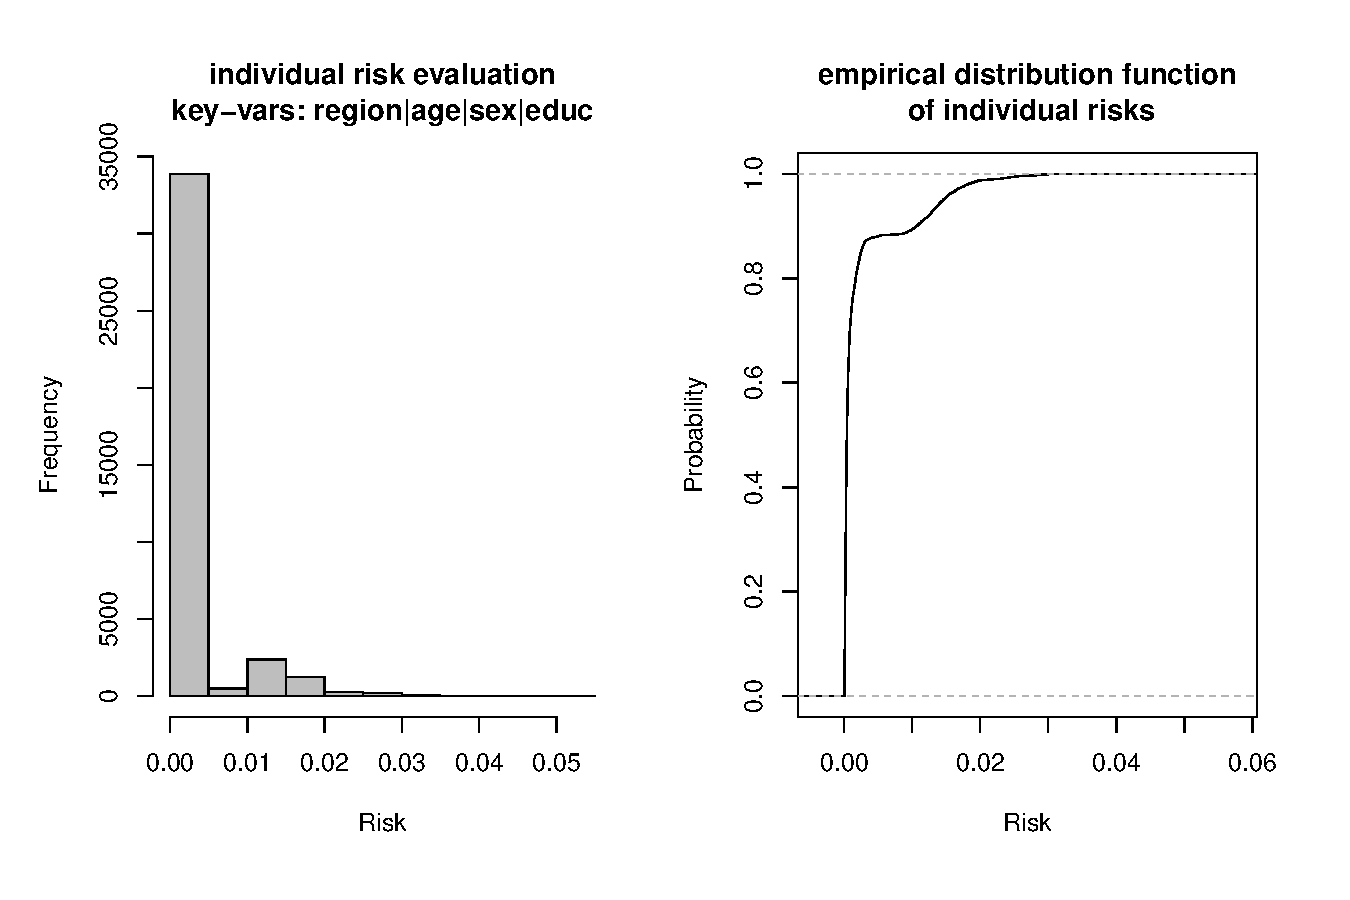
\includegraphics[width=0.95\textwidth]{risk1}
	\caption{Risk evaluation of unmodified data given key variables 'region', 'sex', 'age' and 'attained education'.}
	\label{graph:risk1}
\end{figure}

It is now our goal to achieve 3-anonymity which means that at least 3 units need to contribute to each key. 
To accomplish this goal we have several possibilities. One possibility is to recode key variables in order to 
reduce the number of keys. Having a look at the key variables we choose it makes sense to reduce the number 
of characteristics for variables age and attained education since these variable have a lot of
 characteristics. Listing~\ref{listing:recoding:keys} shows how to recode variable 
 'z2021\textunderscore h\textunderscore age' into 10-year age categories and reducing information 
 in variable 'z2041\textunderscore h\textunderscore educ' by combining categories.

\begin{lstlisting}[captionpos=b, caption={Recoding of key variables}, label=listing:recoding:keys]
a <- dat$z2021_h_age; v <- dat$z2041_h_educ

# recode age
a <- globalRecode(a, seq(9,99,10), 1:9) 

# recode education
v[v %in% c(6,53,58)] <- 0
v[v %in% 60:69] <- 6
v[v %in% 70:79] <- 7

dat$z2021_h_age <- a; dat$z2041_h_educ <- v	

fk <- freqCalc(dat, keyVars, weightVar)
rk <- indivRisk(fk, survey=TRUE)
\end{lstlisting}

In lines 1 and 2 of Listing \ref{listing:recoding:keys} we create local copies of the variables 'z2021\textunderscore h\textunderscore age' and 'z2041\textunderscore h\textunderscore educ'. Line 4 shows how to apply function \lstinline{globalRecode()} to create 10-year age categories from an integer scaled variable. In this case the first age group is 10-19 years, the second group ranges from 20-29 years. In lines 7 to 9 it is shown how to recode the educational status. In line 5, characteristics 6, 53 and 58 for which no formal description is given are combined with characteristic 0 (no grade completed). In line 8, characteristics 60 to 69 which all represent some kind of bachelor degree are combined into a new category (6). A similar approach is taken in line 9 where characteristics 70 to 79 which represent some kind of post graduation are combined into a new single category (7). In line 11, the original variables in the microdata set are finally replaced with the recoded variables ''a'' and ''v'', respectively while in lines 12 and 13 the frequency and risk-calculations based on the recoded key variables is done.\\

The recoding greatly reduces the number of possible combinations of the key variables. 
We can observe that the number of key that are occupied by one or two households is much lower as it is shown in Listing \ref{listing:results:freq2}.  \\  

\begin{lstlisting}[numbers=none,captionpos=b, caption={Results of frequency calculation after recoding}, label=listing:results:freq2]
print(fk)
231 observation with fk=1 
270 observation with fk=2 
\end{lstlisting}

%pdf("risk2.pdf", width=9, height=6)
%par(mfrow=c(1,2))
%par(oma=c(1,1,1,1))
%hist(rk$rk, col="grey", main="individual risk evaluation\nkey-vars: %region|age|sex|educ", xlab="Risk", ylab="Frequency")
%plot(ecdf(rk$rk), main="empirical distribution function\n of individual risks", %xlab="Risk", ylab="Probability")
%dev.off()
\begin{figure}
	\centering
	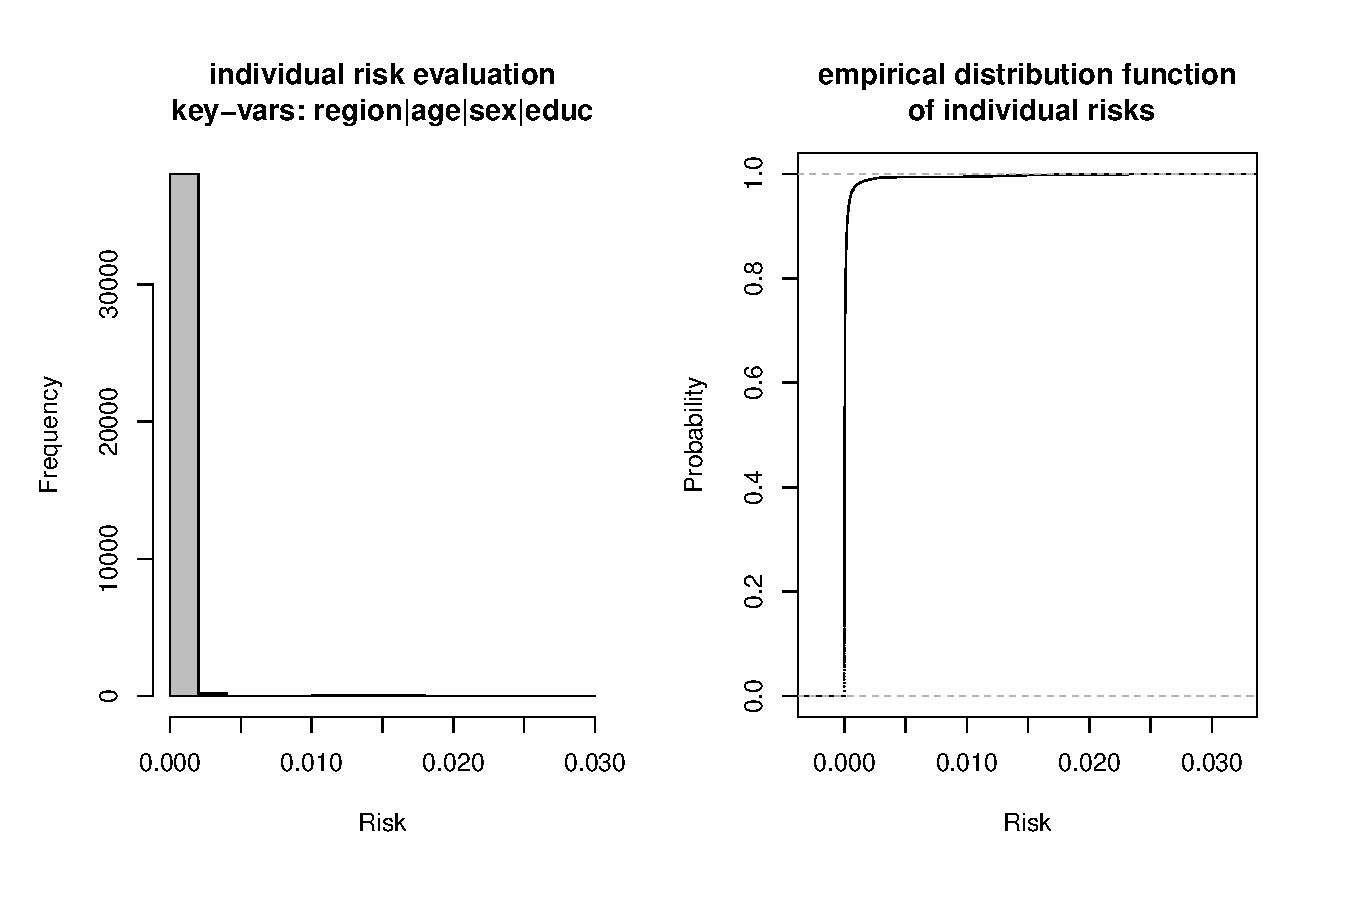
\includegraphics[width=0.95\textwidth]{risk2}
	\caption{Risk evaluation of data given key variables 'region', 'sex', 'age' and 'attained education' after reducing categories through recoding.}
	\label{graph:risk2}
\end{figure}

Having a look at Figure \ref{graph:risk2} we learn that also the individual risk have been reduced through recoding. However, the goal of 3-anonymity is not yet reached. Therefore it is required to suppress values of certain units in the key variables to obtain a dataset in which at least 3 units contribute to every possible key. Using \sdcMicro~this can easily be achieved by using function \lstinline{localSupp()} which is shown in Listing \ref{listing:3-anonymity}.

\begin{lstlisting}[captionpos=b, caption={Achieving 3-anonymity}, label=listing:3-anonymity]
# local Suppression for key-variable 'z2041_h_educ'
lSupp <- localSupp(fk, keyVars[4], rk$rk, threshold=0.004)
fk <- freqCalc(lSupp$freqCalc, keyVars, weightVar)
rk <- indivRisk(fk, survey=TRUE)

# use same approach for other key variables!
\end{lstlisting}

%# code fuer 3-anonymization!
%# educ
%lSupp <- localSupp(fk, keyVars[4], rk$rk, threshold=0.004)
%fk <- freqCalc(lSupp$freqCalc, keyVars, weightVar)
%rk <- indivRisk(fk, survey=TRUE)
%length(which(is.na(lSupp$freqCalc[,keyVars[4]])))
%
%# Age
%lSupp <- localSupp(fk, keyVars[3], rk$rk, threshold=0.002)
%fk <- freqCalc(lSupp$freqCalc, keyVars, weightVar)
%rk <- indivRisk(fk, survey=TRUE)
%length(which(is.na(lSupp$freqCalc[,keyVars[3]])))
%
%# sex
%lSupp <- localSupp(fk, keyVars[2], rk$rk, threshold=0.001)
%fk <- freqCalc(lSupp$freqCalc, keyVars, weightVar)
%rk <- indivRisk(fk, survey=TRUE)
%length(which(is.na(lSupp$freqCalc[,keyVars[2]])))
%
%# region
%lSupp <- localSupp(fk, keyVars[1], rk$rk, threshold=0.001)
%fk <- freqCalc(lSupp$freqCalc, keyVars, weightVar)
%rk <- indivRisk(fk, survey=TRUE)
%length(which(is.na(lSupp$freqCalc[,keyVars[1]])))

With respect to Listing \ref{listing:3-anonymity} we start dealing 
with key-variable 'z2041\textunderscore h\textunderscore educ'. In lines 2 we 
suppress the values of all units that have an individual risk that is larger than 0.004. The threshold of 0.004 is
motivated from the histogram and the empirical cummulative distribution plot in the right graphic of Figure~\ref{graph:risk2}. 
In such a plot one can see the distribution of the risk and it is resonable to set a threshold that separates the main bulk of the data with the
risky data. Note, that their exists no general definition of the threshold, and also legal aspects could play 
a role to determine the threshold, i.e. for highly sensitive data a lower threshold might be chosen than for data 
which seems to include no highly confidential information.

In line 3 we re-calculate the frequencies based on the data set with suppressions and 
calculate the corresponding individual reidentification risks in line 4. \\

The same approch is repeated for the other key variables with the only difference 
being the value of the threshold that should be used for suppressing values. 
We note that the individual risks for each unit can be accessed from objects calculated
 with function \lstinline{indivRisk()} and the value of the threshold can again be specified explorative at a plot showing
 the empirical cummulative distriubtion function as in the right graphic of Figure~\ref{graph:risk2}. 
 After suppressing values for each of the four 
 key variables, we observe that we have reached our 
goal of $k$-Anonymity as it is shown in Section~\ref{listing:results:freqAnon}.
\begin{lstlisting}[numbers=none,captionpos=b, caption={Results of frequency calculation after local suppression}, label=listing:results:freqAnon]
0 observation with fk=1 
0 observation with fk=2 
\end{lstlisting}
We now have reached 3-anonymity within the selected subset of key variables but
we had to suppress values. A total of 251 values were suppressed in variable
z2041\textunderscore h\textunderscore educ, 117 values have been suppressed in z2021\textunderscore h\textunderscore age, 93 values in z2011\textunderscore h\textunderscore sex and 4 values had to be removed in w\textunderscore regn. We note that \sdcMicro~also provides a function that allow to reach $k$-Anonymity automatically. For a detailed information the interested reader is suggested to have a look at the corresponding help file \lstinline{?localSupp2Wrapper}.

%pdf("risk3.pdf", width=9, height=6)
%par(mfrow=c(1,2))
%par(oma=c(1,1,1,1))
%hist(rk$rk, col="grey", main="individual risk evaluation\nkey-vars: %region|age|sex|educ", xlab="Risk", ylab="Frequency")
%plot(ecdf(rk$rk), main="empirical distribution function\n of individual risks", %xlab="Risk", ylab="Probability")
%dev.off()

\begin{figure}
	\centering
	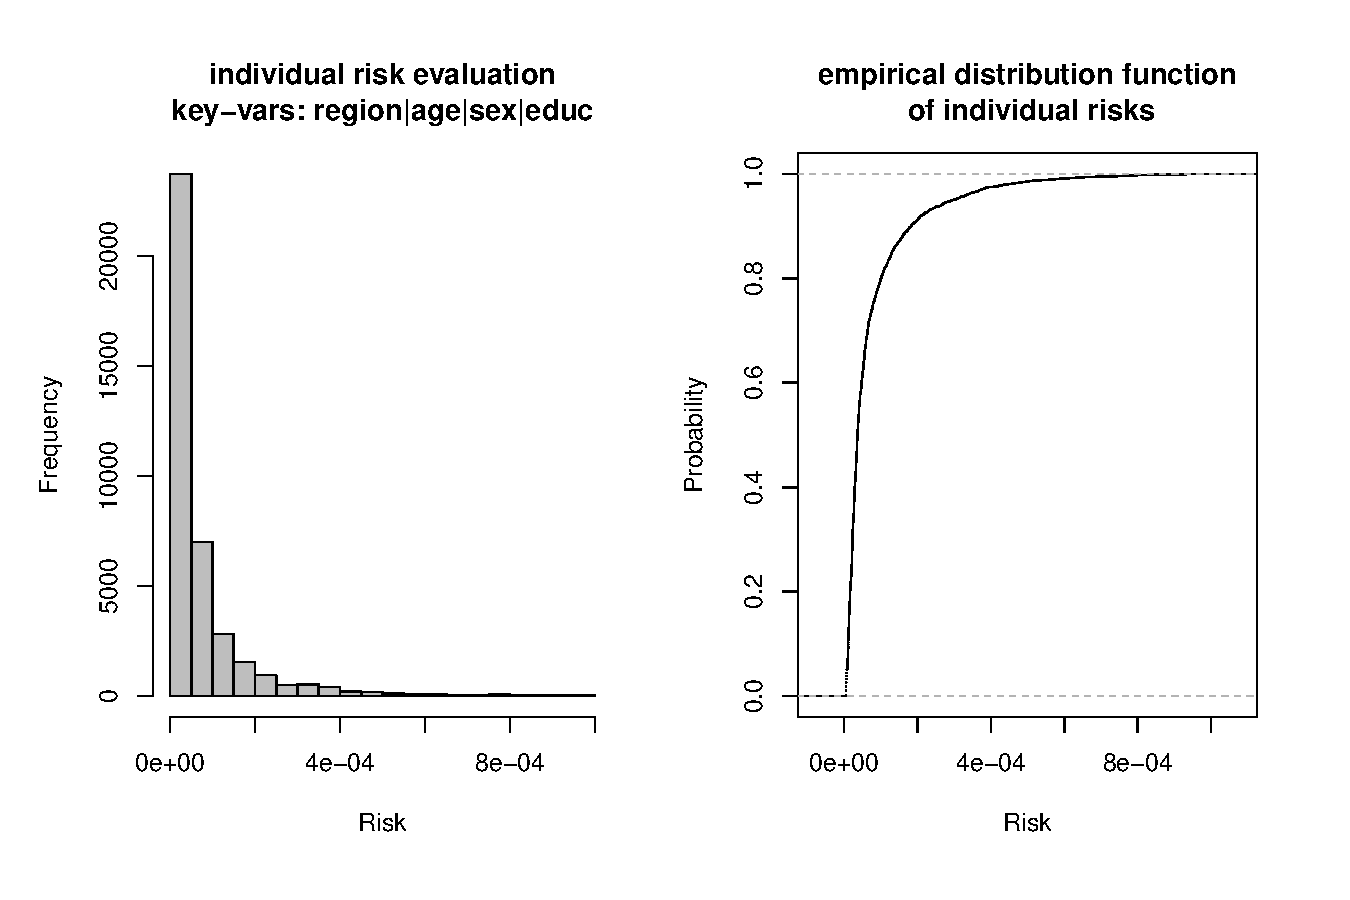
\includegraphics[width=0.9\textwidth]{risk3}
	\caption{Risk evaluation of data given key variables 'region', 'sex', 'age' and 'attained education' after recoding and local suppression.}
	\label{graph:risk3}
\end{figure}

Figure \ref{graph:risk3} clearly shows the reduced risk of reidentification of households compared to Figure \ref{graph:risk1} after performing both global recoding and local suppression to achieve 3-anonymity. \\

We now continue and work to protect confidential numerical variables. 
In this microdata set, we decide that all variables containing information on 
income should be deemed confidential and thus be additionally protected while 
numerical variables containing information on expenditures are not confidential. 
To protect numerical confidential variables one could use function 
\lstinline{microaggregation()} as shown in Listing \ref{listing:microAgg}. 

\begin{lstlisting}[captionpos=b, caption={Microaggregation for confidential numerical variables}, label=listing:microAgg]
mInd <- c(654:670, 671:681, 693:714)
m <- dat[,mInd] 
mDat <- microaggregation(m, method = "mdav", aggr = 3)
dat[,mVars] <- mDat$mx 
\end{lstlisting}
In the first line of Listing \ref{listing:microAgg} we define the 
columns that contain variables dealing with any kind of income. In the second line 
we create a subset of the microdata set that only contains these confidential variables. 
In line 3 we apply function \lstinline{microaggregation()} using method 'mdav' 
which forms the proximity using a multivariate distance method and calls a \texttt{C++} 
implementation written by the International Household Survey Network (IHSN).
Parameter aggr=3 is set to 3 so that proximities of size 3 are generated. Note that from size 3 automatically 
$3$-anonymity is created, i.e. always three observations have the same values in the mircoaggregated variables. 
More protection is guaranteed if the aggregation level is increased but the data utility will be decreased at the same time.
In the last line we map the microaggregated data set back to the original microdata set by simply replacing the non-microaggregated variables by their microaggregated counterparts.\\

It is now of course possible to add another layer of uncertainty to the data set by stochastically changing 
characteristics of some (categorical) variables using post-randomization with 
function \lstinline{pram()} as it is shown in Listing \ref{listing:pram}.
\begin{lstlisting}[captionpos=b, caption={Post randomization for a categorical variable}, label=listing:pram]
vInd <- match('z2031_h_ms', colnames(dat))
pr <- pram(dat[,vInd], pd=0.85)
dat[,vInd] <- pr$xpramed
\end{lstlisting}
In the first line of Listing \ref{listing:pram} the column index of the variable 
'z2031\textunderscore h\textunderscore ms' containing maritial status is calculated. 
In the second line the actual post randomization is performed. 
The parameter 'pd' is set to 0.85 which means that on average around 85\% of the variable 
characteristics should not change. Decreasing this parameter value more values are changed  to
other categories and the data utility decreases as well as the disclosure risk. Again, this parameter should be specified
on legal basis, i.e. the need for changing more values than 0.15 \%, for example, should be 
argued by lawyers that can decide how many 
changes are sufficient so that an intruder is (enough) unsure if the value is true or not.


The transition matrix itself is internally calculated. 
The resulting output object 'pr' contains besides the transition 
matrix and the original input vector also the modified, post-randomized vector. 
In the third line we replace the original characteristics of variable 
'z2031\textunderscore h\textunderscore ms' by its post-randomized version. \\

We can now state that we have created a microdata set that features 
3-anonymity within the selected set of key variables that has low individual 
reidentification risks and that has been microaggregated in all variables that 
contain information on any sort of income which we defined as confidential. 
Additionally we have post-randomized another categorical variable. 
After performing these steps it would be the task of the subject matter 
specialists or people responsible to decide if the modified microdata set is safe 
to be published. If this is the case, the file could be published. 
If not, additional disclosure limitation techiques such as adding noise 
(using \lstinline{addNoise()}) should be done or the information of the 
microdata set could be even more reduced by suppression, recoding, 
post-randomization or any other method. 


%Part I. Identification and Other Information
%  (Geographic Identification, Other Information and Particulars about the Family)
% 
% Part II.    Expenditures
%		Section A.  Food, Alcoholic Beverages and Tobacco 
%		Section B.  Fuel, Light and Water, Transportation and Communication, Household Operations
%		Section C.  Personal Care and Effects, Clothing Footwear and Other Wear
%		Section D.  Education, Recreation, and Medical Care
%		Section E.  Furnishings and Equipment
%		Section F.  Taxes
%		Section G.  Housing, House Maintenance and Minor Repairs
%		Section H.  Miscellaneous Expenditures
%		Section I.   Other Disbursements 
%  
%Part III.   Income
%	Section A.  Salaries and Wages from Employment
%	Section B.  Net Share of Crops, Fruits and Vegetables Produced and/or Livestock and Poultry Raised by Other Households
%	Section C.  Other Sources of Income
%	Section D.  Other Receipts
%	Section F.  Family Sustenance Activities 
% 
% Part IV.   Entrepreneurial Activities
%	Section A1.  Crop Farming and Gardening
%	Section A2.  Livestock and Poultry
%	Section A3.  Fishing
%	Section A4.  Forestry and hunting
%	Section A5.  Wholesale and Retail
%	Section A6.  Manufacturing
%	Section A7.  Community, Social, Recreational and Personal Services
%	Section A8.  Transportation, Storage and Communication Services
%	Section A9.  Mining and Quarrying
%	Section A10.  Construction
%	Section A11.  Entrepreneurial Activities Not Elsewhere Classified 


\subsection{Application to SES data}\label{app:ses}

%\begin{lstlisting}[numbers=none,captionpos=b, caption={Loading the SES data.}, label=listing:loadses]
%library(sdcMicro)
%load('../Daten/pop2.RData')
%\end{lstlisting}


First, the original microdata have to be loaded into \proglang{R} as shown in Listing~\ref{listing:loadses2}.

\begin{lstlisting}[numbers=none,captionpos=b, caption={Loading the SES data.}, label=listing:loadses2]
load("ses.RData")
\end{lstlisting}

The result of this step is an object 'x' that exists in the current workspace of \R~that contains the original, unmodified SES data.

\subsubsection{Key Variables for Re-Identification} \label{suub:keys}

Again no direct identifiers are included in the data. 
The identification of an enterprise may leads to information about their employees.

For the categorical key variables at employment level the following variables are selected \citep[see also][]{ichim07}: 
\begin{itemize}
	\item {\bf Size}: size of the enterprise
	\item {\bf age}: age in years
	\item {\bf Location}: geographic location with 3 categories
	\item {\bf economicActivity}: the economic branche of the corresponding work centre given as NACE Rev. 2 - 
	Statistical classification of economic activities
\end{itemize} 

    
As continuous key variables at employment level the following variables are selected:
\begin{itemize}
	\item {\bf earnings}: 
gross earnings 
%   \item {\bf special payments}:
%special payments
   \item {\bf hourly earnings}: generated from earnings and hours paid in Listing~\ref{listing:sesrecode1}.
\end{itemize}


\subsubsection{Pre-processing Steps}

Some important variables have to be constructed first. The variable that contains information on gender is recoded, the earnings per hour are constructed from earnings and hours paid, and the variable 'age' has to be calculated from the year of birth. Listing~\ref{listing:sesrecode1} shows how to perform these steps:

\begin{lstlisting}[numbers=none,captionpos=b, caption={Pre-processing of the SES data to generate new variables.}, label=listing:sesrecode1]
x$Sex <- factor(ifelse(x$Sex=='Male','male','female'))
x$earningsHour <- x$earningsMonth / x$hoursPaid
x$age <- 2006 - x$birth
\end{lstlisting}

\subsubsection{Risk Estimation}
Now we are ready to estimate the disclosure risk of our data corresponding to the key variables that have been defined.
In Listing \ref{listing:freq1} it is shown how to set up the disclosure scenario for the SES data. In this code we calculate the column-indices of the key-variables (variable 'keyEC') and the variable containing sampling weights (variable 'wVar').

\begin{lstlisting}[numbers=none,captionpos=b, caption={Frequency and risk estimation of the raw SES data.}, label=listing:seskey]
## categorical key-variables
keyVars <- c('Size', 'age', 'Location', 'economicActivity')
keyEC <- match(keyVars, colnames(x))
wVar <- match('GrossingUpFactor.y', colnames(x))
fr2 <- freqCalc(x, keyVars=keyEC, w=wVar)
fr2
 --------------------------
4979 observation with fk=1 
6312 observation with fk=2 
 --------------------------
rk <- indivRisk(fr2)
rk

method=approx, qual=1
 --------------------------- 
37697 obs. with much higher risk than the main part
\end{lstlisting}

It is easy to see the large number of unique combinations from cross-tabulating the 
categorical key variables (\texttt{fk$=1$} in Listing~\ref{listing:seskey}). Also a huge number of 
observations have a considerable higher risk (esitmated at population level) than the main part of the data.

\subsubsection{Recoding and Local Suppression}

It is therefore necessary to recode some categories of the key variables to receive a lower number of uniqueness.
This is done in Listing~\ref{listing:sesRecode}. Here, the NACE classification is changed from 2-digit codes to 1-digit codes, whereas
the aggregation of the classifications are based on expert knowledge, i.e. those categories are combined where the economic branches 
are similar.
Next, the categories of the size of the enterprises is reduced. Finally, the age of the employees are categorized in six age classes.

% save(fr, file="fr-scenario1.RData")
% load("fr-scenario1.RData")


%save(fr2, file="fr-scenario2.RData")
%load("fr-scenario2.RData")

\begin{lstlisting}[numbers=none,captionpos=b, caption={Recoding economic activity, size and age.}, label=listing:sesRecode]
## recode economic activity
library(stringr)
a <- as.character(x$economicActivity)
ecoANew <- rep('Q-ExtraTerr', nrow(x))
ecoANew[a %in% str_c('R', 10:14)] <- 'C-Mining'
ecoANew[a %in% str_c('R', 15:37)] <- 'D-Manufacturing'
ecoANew[a %in% str_c('R', 38:44)] <- 'E-Electricity'
ecoANew[a %in% str_c('R', 45:49)] <- 'F-Construction'
ecoANew[a %in% str_c('R', 50:54)] <- 'G-Trade'
ecoANew[a %in% str_c('R', 55:59)] <- 'H-Hotels'
ecoANew[a %in% str_c('R', 60:64)] <- 'I-Transport'
ecoANew[a %in% str_c('R', 65:69)] <- 'J-FinancialIntermediation'
ecoANew[a %in% str_c('R', 70:74)] <- 'K-RealEstate'
ecoANew[a %in% str_c('R', 75:79)] <- 'L-Public'
ecoANew[a %in% str_c('R', 80:84)] <- 'M-Education'
ecoANew[a %in% str_c('R', 85:89)] <- 'N-Health'
ecoANew[a %in% str_c('R', 90:94)] <- 'O-Other'
ecoANew[a %in% str_c('R', 95:98)] <- 'P-Households'
x$economicActivity <- ecoANew; rm(ecoANew,a)

## recode size classes:
levels(x$Size) <- list(E10_49=c('E10_49'), E50_249='E50_49', E250plus=c('E250_499','E500_999','E1000')) 
		
## recode age		
x$age <- cut(x$age, breaks=c(0,19,29,39,49,59,120))
\end{lstlisting}

%save(frAfter, file="frAfter-scenario1.RData")
%load("frAfter-scenario1.RData")

After performing the recoding of key variables we can calculate the new frequencies as it is shown in Listing~\ref{listing:sesscenario2b}.

\begin{lstlisting}[numbers=none,captionpos=b, caption={Frequency calculation based on the recoded variables.}, label=listing:sesscenario2b]
### Disclosure Scenario 2 (after recoding of key-variables)
fr2After <- freqCalc(x, keyVars=keyEC, w=wVar)
 --------------------------
0 observation with fk=1 
0 observation with fk=2 
 --------------------------
rk <- indivRisk(fr2After)
max(rk$rk)
[1] 0.0006009207
\end{lstlisting}

In general there are at least four possiblities to archieve $k$-anonymity. The first possibility is to randomized the values of a categorical variable 
with the help of function \lstinline{pram()}, as shown in Section~\ref{method:pram}. An alternative way could be to delete some values randomly and impute those values in a proceeding step.  

Another possibility is to apply further recodings, for example, to 
allow fewer categories for the economic activity. The last possiblity is to apply local suppression as it was already shown in Listing \ref{listing:3-anonymity}. In this case however it is not required to take any further steps since we learn from the output of function \lstinline{freqCalc()} that 3-anonymity has already been reached with the recoding that has already been done since the number of observations with 'fk' being one or two is zero. We also see that the maximal risk for re-identification is very low.

However, for the sake of completeness we list the three functions of \sdcMicro~that can used to perform local suppression. Function \lstinline{localSupp()} can be used to suppress all values for a given key variable for all units which have a risk that is higer a specified threshold value. This value can be set when calling the function.  

The other functions are \lstinline{localSupp2()} and \lstinline{localSupp2Wrapper()} that work slightly different. Both functions provide a heuristic algorithm that performs local suppression repeatedly until $k$-anonymity is reached. It is also possible to specify an importance vector that is taken into account when suppressing values in the key variables. It is therefore even possible to specify the importance of key variables in a way that no information is removed for these variables.

\subsubsection{Perturbing the Continuous Scaled Variables}

A bunch of methods are available to perturb continuously scaled (key) variables.

In the Listing~\ref{listing:sesNum1} it is shown how to apply microaggregation as well as adding (correlated) stochastic noise to continuously scaled variables. In this example the {\it mdav} method for microaggregation is used. The parameter \texttt{aggr} determines how many observations are always considered together when performing the aggregation. 

\begin{lstlisting}[numbers=none,captionpos=b, caption={Microaggregation and addition of stochastic noise applied to continuous key variables of the SES data.}, label=listing:sesNum1]
numVars <- c('earningsHour', 'earnings')
cInd <- match(numVars, colnames(x))

## perform microaggregation
x[,cInd] <- microaggregation(x[,cInd], method='mdav', aggr=3)

## add correlated noise
x[,cInd] <- addNoise(x[,cInd], method='correlated')
\end{lstlisting}

In Listing~\ref{listing:sesNum1} we show how to use function \lstinline{addNoise()} to add correlated noise to numerical key variables. In this case it is required to set parameter {\tt method='correlated'} when calling the function. We note that quite a few different methods for noise-addition - even methods that takes the structure of outlying observations into account - can be selected in function \lstinline{addNoise()}.

%\begin{lstlisting}[numbers=none,captionpos=b, caption={Adding correlated noise to %the continuous key variables of the SES data.}, label=listing:sesNum1]
%x[,colInd] <- addNoise(x[,colInd], method='correlated')
%\end{lstlisting}



%%%%%%%%%%%%%%%%%%%%%%%%%%%%%%%%%%%%%%%%%%%%%%%%%%%%%%%%%%%%%%%%%%%%%%%%%%%%


%\section{Aim of this Report}
%
%The goal of this project is both to integrate existing \texttt{C++} code from the OECD 
%into the \proglang{R} package \pkg{sdcMicro} 
%\citep{sdcMicro,templ08tdp,Templ09tdp,templ11book} 
%and to draft guidelines 
%for the application of statistical disclosure control methods to perturbe 
%microdata for anonymisation of the orginal data.
%
%Section~\ref{sec:imp} discusses some details about the implementation of the methods. Section~\ref{sec:bench} describes the
%benchmarking indicators from where the disclosure methods are evaluated with measures described in Section~\ref{sec:utiltiy}.
%Section~\ref{sec:results} shows the results based on the benchmark indicators and utility measures. 
%The last section, Section~\ref{sec:conclusion} concludes.
 %
  %
%


\section{Anonymised Data and Measuring the Risk} \label{sec:risk}

The data has been anonymised by recoding, suppression, by pram and by microaggragatin and adding noise. For details, have a look in the third 
deliverable of the project \citep{Meindl12del3}.

The risk measurement can only be done for recoding and local suppression (by using the the $k$-anonymisty approach and/or the 
risk framework of \cite{Rinott06} or \cite{manning08}) 
and methods that perturbe continous variables (using the function \lstinline{drisk()} in \proglang{R} \citep{Templ08d,Templ08f} 
package \pkg{sdcMicro}). Rank swapping or pram
change values randomly and the risk of re-identification have to be evaluated by eperts on laws, i.e. a 
threshold, how many swapped values are enough so that an intruder have an uncertainty if a re-idenfication is wrong or not, has to be fixed.

In Section~\ref{sec:results} we evaluate anonymised data that fulfills $k$-anonymity, and using the default parameters 
of \pkg{sdcMicro} for \lstinline{pram} and rank swapping.


\section{Utility Measures} \label{sec:utility2}
After performing the task of anonymizing micro data it is alway neccessary to
assess the quality of the resulting micro data set. 

As mentioned in Section~\ref{sub:ut} anonymised data are usually 
evaluated using very generally defined utility measures such as differences in means or covariances.
We also mentioned there that the evaluation of the data utility of anonymised data should better be 
based on those (benchmarking) statistics/indicators that are most important to estimate from the data. 

For FIES and SES, this includes that famous indicators like the GINI coefficient (see Equation~\ref{Equ:gini}),
but also model-based estimations that are typically applied on the data should be precise as possible.
In addition, in the following we also evalute the methods based on overlaps in confidence intervals which 
has - to our knowledge - never been done in literature, but it seems to be very reasonable to look also if the variances of 
the estimates are preserved.
%Usually, only point estimates are compared.
And there is another reason to do that. When considering the variances of the estimates obtained from original data and anonymised data allows 
to take the sample size into account. \\


We now continue to describe
how one can achieve the goal of evaluating the quality of the results. It should
be also noted that it may be neccessary to perform the quality assessment
multiple times to be able to compare different anonymization methods. This
allows the SDC specialist to decide on an anonymization technique that not only
leads to protected micro data but also to data that still feature high data
quality.


The utility measures chosen, which are in the calculated on the benchmarking indicators defined in
Appendix~\ref{sec:ind}, are the following 
\begin{itemize}
  \item about the difference in the estimation of the Gender Pay Gap (GPG)
and the GINI coefficient from the original and perturbed data defined for $h$ domains:
\begin{equation}
ARB = \frac{|\frac{1}{h} \sum_{i=1}^{h} (\hat{\theta}_i - \theta_i)|}{\theta_i}
\quad.
\end{equation}
\item
Additionally, one model is
predicted (see Appendix~\ref{appendix:mod}) and from the predicted values the 
indicator of interest (e.g. the GINI) is 
estimated.
\item
Moreover, the variances are estimated and the \textbf{overlap of the confidence
intervals} of the perturbed and original data is evaluated and reported in
percentages (of overlap).
\end{itemize}


In Section \ref{sec:results} we show how to assess data utility for some
important indicators for the SES data set. 

\section{Results} \label{sec:results}


\subsection{ARB}
Table~\ref{tab:gpg} shows the ARB whereas the overall
estimate is shown and the mean over the domain (sex $\times$ age class) estimates.
It is easy to see that microaggregation ('ma'; here method 'mdav' from package \pkg{sdcMicro} \cite{sdcMicro,Templ08tdp} was chosen) 
provides much better
results than the correlated noise method \cite{Brand04} using the default parameters of \pkg{sdcMicro}. 
%The
%overlap in the confidence intervals is zero for the correlated noise method. 
The ARB estimates are the same for recoding, pram or swapped variables since the 
GPG is estimated only from the microaggregated 
hourly earnings. However, recoding, swapping and pram influences 
the model estimates since the age is categorized or swapped.
Hereby, recoding provides better results than pram and swapping (see also Table~\ref{tab:gini} 
for similar results on the Gini coefficient). It can also be seen that the ARB is small when recoding and microaggregation
were applied to anonymise the data. The model-based estimates become worst when swapping techniques like numerical rank swapping 
or pram are additionally applied.


\begin{table}[ht]
\begin{center}
\caption{\label{tab:gpg}Comparison of different methods using the absolute Relative Bias (ARB) in gender pag gap. 
The .m indicates that the estimates based on models (see Appendix B.3), the h. indicates that the estimates is based on domain level.\vspace{0.2cm}}
\begin{tabular}{rrrrr}
  \hline
 & ARB & ARB.m & h.ARB & h.ARB.m \\ 
  \hline
recode+noise & 46.73 &  & 126.02 &  \\ 
  recode+ma & 0.02 & 0.30 & 0.03 & 6.11 \\ 
  recode+pram+ma & 0.02 & 22.13 & 0.03 & 14.46 \\ 
  recode+swap+ma & 0.02 & 12.84 & 0.03 & 6.44 \\ 
  pram+ma & 0.02 & 14.60 & 0.03 & 10.77 \\ 
  swap+ma & 0.02 & 11.76 & 0.03 & 8.56 \\ 
   \hline
\end{tabular}
\end{center}
\end{table}

% latex table generated in R 2.13.0 by xtable 1.5-6 package
% Fri Apr 27 10:43:36 2012
\begin{table}[ht]
\begin{center}
\caption{\label{tab:gini}Comparison of different methods using the absolute Relative Bias (ARB) of the Gini coefficient. 
The .m indicates that the estimates based on models (see Appendix B.3), the h. indicates that the estimates is based on domain level.\vspace{0.2cm}}
\begin{tabular}{rrrrr}
  \hline
 & ARB & ARB.m & h.ARB & h.ARB.m \\ 
  \hline
recode+noise & 1.12 &  & 16.37 &  \\ 
  recode+ma & 0.02 & 0.07 & 0.07 & 6.11 \\ 
  recode+pram+ma & 0.02 & 41.95 & 0.07 & 14.46 \\ 
  recode+swap+ma & 0.02 & 34.16 & 0.07 & 6.44 \\ 
  pram+ma & 0.02 & 35.69 & 0.07 & 10.77 \\ 
  swap+ma & 0.02 & 34.22 & 0.07 & 8.56 \\ 
   \hline
\end{tabular}
\end{center}
\end{table}

\subsection{Overlap in Confidence Intervals}
By estimating the confidence interavals (for the gender pay gap, for example) one can also 
have look at the overlap of the confidence interval
of a parameter estimated from the perturbed and the original data.

This can be done using the following lines of code shown in Listing~\ref{listing:ci}.
First the Gini coefficient and its variance (for more details on variane estimation see Appendix~\ref{appB}) 
is estimated from both, the original data and the anonymised data. The confidence intervals are 
very similar and almost completely overlaps. This is also true when displaying the confidence intervals by stratum
(this is saved in object \texttt{v1} and \texttt{v1a}).

\begin{lstlisting}[frame=single, label=listing:ci, caption={Overlap in confidence intervals from estimates based on perturbed and original data.}] 
library(laeken)
# we take one stratum (for computational speed) and full time employees
x <- x[x$economicActivity=="R14" && x$FullPart=="FT",]
dim(x)
[1] 1554   43  ## number of observations and variables used

## gini from original data
g1 <- gini(inc="earningsHour", weigths="GrossingUpFactor.y", breakdown="education", data=x) 

## gini from perturbed data
g1a <- gini(inc="earningsHourM", weigths="GrossingUpFactor.y", breakdown="education", data=x) 

## corresponding variances
v1 <- variance("earningsHour", weights="GrossingUpFactor.y", data=x, 
		indicator=g1, X=calibVars(x$Location), breakdown="education", seed=123)
v1a <- variance("earningsHourM", weights="GrossingUpFactor.y", data=x, 
		indicator=g1a, X=calibVars(x$Location), breakdown="education", seed=123)	
v1$ci
   lower    upper 
15.31177 19.16410 
v1a$ci
   lower    upper 
15.32402 19.15750 
\end{lstlisting}

But also the differences of the regression coefficients are of interest. Whereas it is not or hardly be possible 
to compare the coefficients obtained from a model based on original data with the coefficients obtained by
recoded data (fewer categories includes other/fewer regression coefficients) it is possible to see the effect of numerical
rank swapping or pram on the regression coefficients.

This is highlighted in Figure~\ref{fig:ci} whereas the overlap of confidence intervals is clearly feasible.




\begin{figure}[ht]
 \centering
 \subfigure[Rank swapping.]{
  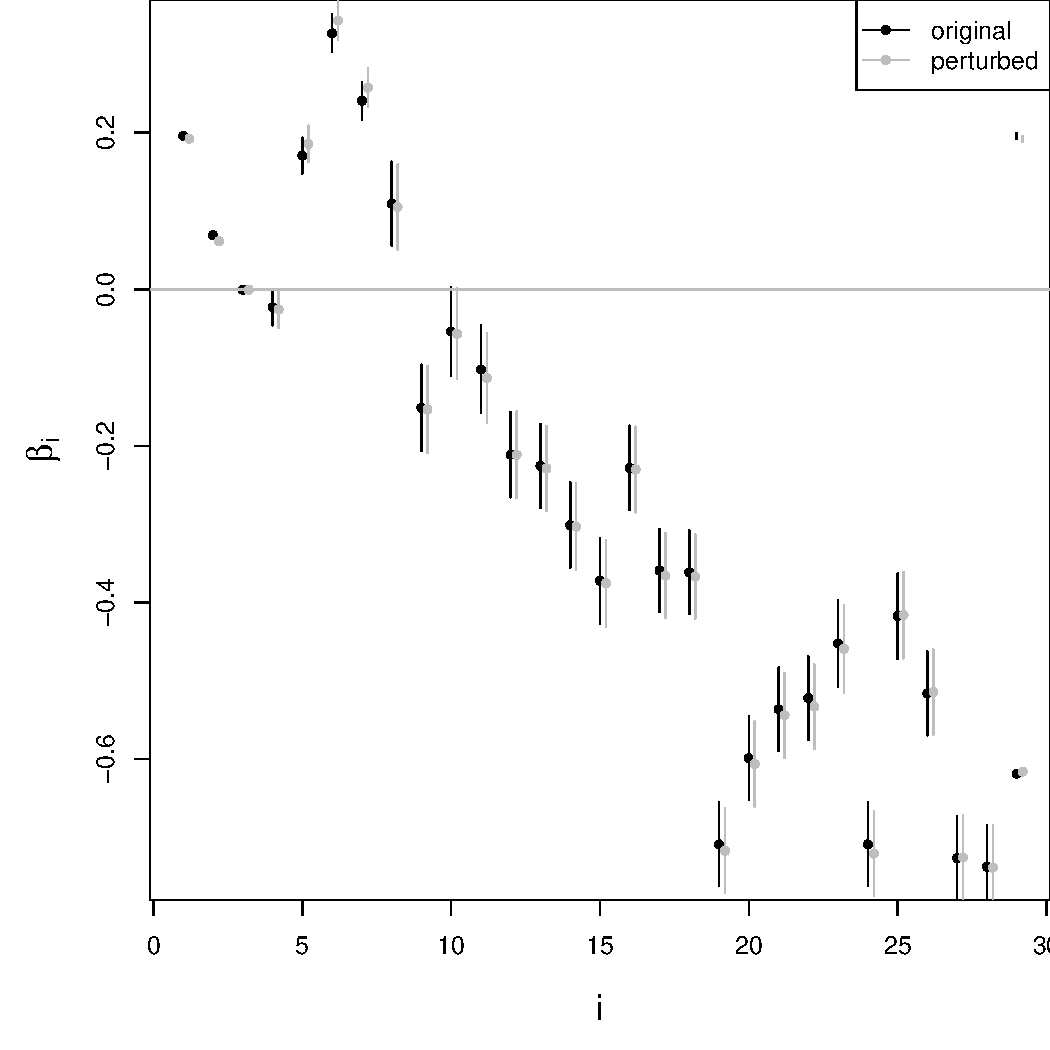
\includegraphics[width=0.45\textwidth]{confintSwap}
   \label{fig:p1}
   }
 \subfigure[Pram using the default parameters.]{
  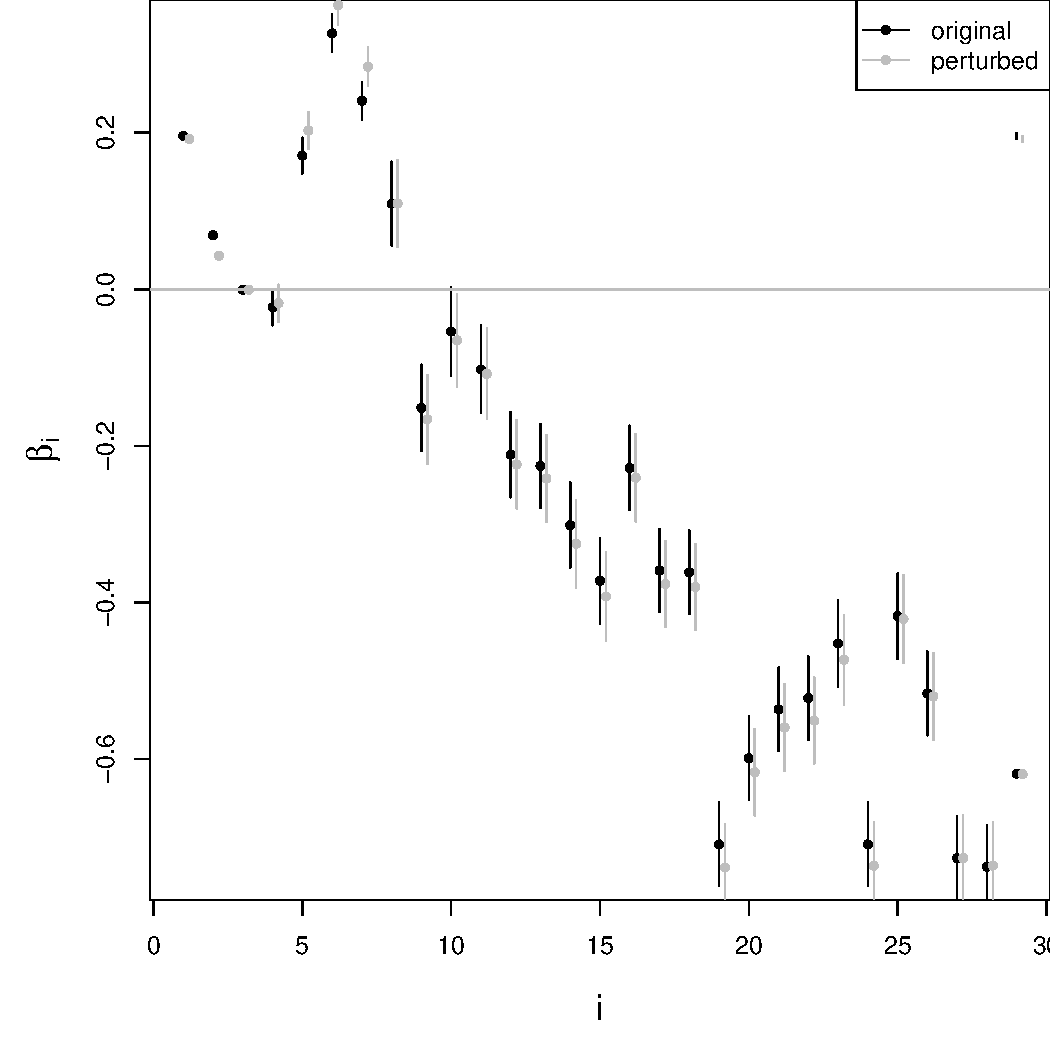
\includegraphics[width=0.45\textwidth]{confintPram}
   \label{fig:p2}
   }
 \caption[]{%
   \label{fig:ci}Confidence intervals for the regression coefficients obtained
  from the model based on original data (black lines) and perturbed data (grey
  lines).}
\end{figure}


%\textcolor{red}{RESULTS FROM FIES DATA ARE MISSING IN THIS DRAFT}


%After selecting a data set, the
%key variables and the vector containing the sampling weights has to be selected once. After selection, automatically all 
%summary statistics (frequencies and disclosure risk) are calculated and displayed. Recoding, suppression, microaggregation 
%or adding noise can be carried out within the present version of the GUI. Figure~\ref{fig:gui2} displays the summary statistics
%after some recodings and local suppression of some key variables.
%
%\begin{figure}[ht]
%\begin{center}
%\caption{\label{fig:gui2}The GUI shows the summary statistics (interactively) of already almost anonymised data.}
%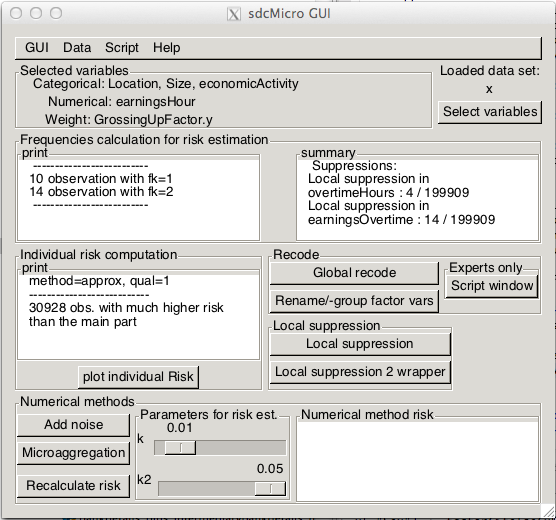
\includegraphics{gui2}
%\end{center}
%\end{figure}
%
%The development of a stable version of the GUI including more methods 
%and it's full documentation corresponding the application to FIES and SES data is future work. 


%\textcolor{red}{SNAPSHOTS OF GUI USING SES OR FIES DATA. EXPLAIN THE SNAPSHOTS. ?????? N}

\newpage
\section{Conclusions} \label{sec:conclusions}







%\section{Conclusions} \label{sec:conclusions}

In this guidelines we have shown basic concepts of how microdata may be modified in
order to generate confidential data that can be released.
 We also showed how to practically implement these concepts using the free and open source \R~package \pkg{sdcMicro}. 
 For this reason these guidelines may prove helpful to subject matter experts that have to deal with the task of preparing safe micro data.

Additional methods are available and described in detail in the \proglang{R} package \pkg{sdcMicro}, such as the suda2 algorithm to
find unique observations on subsets, further recoding facilities as well as a GUI, implemented in \pkg{sdcMicroGUI} \citep{Templ09tdp}.

In general, the following recommendations are given:
\paragraph{Recommendation 1:} Carefully choose the set of variables that are disclosive using knowledge of both subject 
matter experts and disclosure control experts. 

\paragraph{Recommendation 2:} Always perform a frequency- and risk estimation in order to evaluate how many observations have a high risk of dislosure.

\paragraph{Recommendation 3:} Apply recodings to reduce uniqueness given the set of categorical key variables.
This approach should be done in an explorative manner.
However, recodings on a variable should also be based on expert knowledge to combine categories that are reasonable to combine.
Alternatively, swapping procedures may
be applied on the categorical key variables so that data intruders can not be
certain anymore if an observation has or has not been perturbed.

\paragraph{Recommendation 4:} If recoding was applied, suppress the last remaining values to obtain $k$-anonymity.

\paragraph{Recommendation 5:} Apply microaggregation to continuously scaled key variables. This automatically provides $k$-anonymity within those variables.

\paragraph{Recommendation 6:} Quantify the data utility not only on typical estimates (like quantiles or correlations) but also on the most 
important data-specific benchmarking indicators. \\


The results show that recoding and microaggregation works well to obtain non-confidential data with high data quality. 
While the disclosure risk cannot be expressed in statistics for swapping methods like rank swapping or pram, these methods would have 
its advantages when a high number of key variables are chosen, since a high number of key variables leads to a high number of unique cominations that
cannot be significantly reduced by recoding. 

In general, the inclusion of \texttt{C++} code from the OECD leads to significant performance in computatational 
speed of the implementation 
\citep[see][]{Kowarik12del1}. In addition, the package can be used for free without paying 
licences of a statisitical software such as SPSS or STATA.

%A new stable and enriched version of the graphical user interface of \R \ package \texttt{sdcMicroGUI} is future work as well as
%to integrate and testing few IHSN \proglang{C++} code, which is not integrated or tested until now (IHSN code for local suppression, for example).

\section*{References}
\addcontentsline{toc}{section}{Bibliography}
\bibliographystyle{plainnat}
\bibliography{deliverable3}

\appendix 

\section{Detailed data description} \label{annex:data} \label{appA}

\subsection{FIES}\label{data:fies}
The first microdata set that we use to apply popular microdata limitation techniques using 
\sdcMicro~is the \textit{Family Income and Expenditure Survey} (FIES) from 2006 
that has been conducted by the National Statistics Office of the Philippines. 
It is a nationwide survey of households that is the main source of information of data on 
family income and expenditures. \\

\subsubsection{Objectives of FIES}
The objectives of the survey are - among others - to gather information on family income and 
expenditures and related information that affects income and expenditure levels and patterns. 
It is also of great interest to collect information about different sources of income, 
levels of living and spending patterns and also about the degree of inequality among families. \\

For the FIES in 2006, households have been sampled according to a complex sampling design. With respect to the goal of this work which is to draft practical guidelines for creating protected microdata files it is not required to go into details about
the sampling procedure. It is however important to note that sampling weights are available and should be taken into account. \\

The questionnaire was split into four main parts that are listed below:
\begin{itemize}	
	\setlength{\itemsep}{-1mm}
	\item Identification and other Information
	\item Expenditures
	\item Income
	\item Entrepreneurial Activities
\end{itemize}

The required interviews have been conducted face to face by trained interviewers. The reporting unit was the family.
The dataset 
%will be used to explain the application of disclosure limitation methods
features a total of 38483 units for which 721 variables have been measured.

More metadata on the FIES2006 data are available from \href{www.census.gov.ph/nsoda}{www.census.gov.ph/nsoda}, including variable
description. 

%%%%%%%%%%%%%%%%%%%%%%%%%%%%%%%%%%%%%%%%%%%%%%%%%%%%%%%%%%%%%%%%%%%%%%%%%%%
%%%   SES

\subsection{The Structural Statistics on Earnings Survey (SES)}\label{data:ses}


\subsubsection{General Information about SES}

The Structural Earnings Survey (SES) is conducted in almost all European
countries, and the most important figures are reported to Eurostat.
Moreover, also anonymised microdata are sent from most European Union membership countries to Eurostat. 

%In 2006, the sampling frame in Austria consists of 38200 enterprises and 2.2
%5Mio. employees. 

SES is a complex survey of Enterprises and Establishments with more than 10
employees (11600 enterprises in Austria in year 2006), NACE C-O, including a large
sample of employees (Austria: 207.000). 
In many countries, a two-stage design is used whereas
in the first stage a stratified sample of enterprises and establishments on NACE 1-digit level, 
NUTS 1 and employment size range is drawn with large enterprises commonly having higher inclusion probabilities. In stage 2, systematic sampling or simple
random sampling is applied in each enterprise. Often, unequal inclusion
probabilities regarding employment size range categories are used.
Of course, calibration is applied to represent some population
characteristics corresponding to NUTS 1 and NACE 1-digit level, but also 
calibration is carried out for gender (amount of men and womens in the
population).\\

\noindent SES includes information from different perspectives and sources. In
the Austrian case this belongs to:
\begin{description}
\item[Information on enterprise level:]
Question batteries are asked to enterprises like if an
enterprise is private or public or if an enterprise has a collective bargaining
agreement (both binary variables). As a multinomial variable, the kind of
collective agreement is included in the questionnaire.
\item[Information on individual employment level:]
The following questions to employees comes with the standard questionnaire:
social security number, date of being employed, weekly working time,
kind of work agreement, occupation, time for holidays, place of work, gross earning, earning for overtime and amount of overtime.
\item[Information from registers:]  
All other information may come from registers like information about 
age, size of enterprise, occupation, education, amount of employees, NACE and
NUTS classifications.
\end{description}


A detailed information on the SES variables can be found in the appendix.



\subsubsection{Applications and Statistics based on SES}
Every four years the standard publication from national statistical offices is
disseminated after the survey is conducted. In addition, special publications
about low incomes, non-common occupation employment and gender-specific reports are published by some member states \cite[see, e.g.,][]{geissberger10a,geissberger10b}.
Many other national publications from statistical agencies or researchers are
available in almost every country \citep[for some summaries
about publications until 1999,
see][]{Belfield99,Nolan01,Dupray99,frick99,dell00}.


It is interesting to note that anonymised SES 2002 and 2006 data \citep{ses2} from 23 countries can be can be
accessed for research purposes (by means of research contracts) through the safe
centre or anonymised CD-ROM at the premises of Eurostat 
(\href{http://epp.eurostat.ec.europa.eu/portal/page/portal/microdata/ses}{http://epp.eurostat.ec.europa.eu/portal/page/portal/microdata/ses}). 
The output of the users are 
 checked by Eurostat on confidentiality and quality \citep{ses1}.\\
SES Microdata from Czech Republic, Hungary, Ireland,
Italy, Latvia, Lithuania, Netherlands, Norway, Portugal, Slovakia and Spain can also be
analysed via the Piep Lissy remote access system. The user can run 
\texttt{Stata} code on the Piep-Lissy server, whereas some commands
(12 commands in summary) are blocked by the system to prevent listing of individuals. This is, of course not enough to prevent 
re-identification of individuals \citep[see, e.g.,][]{templ11ses}.
The Lissy servers has been intensively used within the EU project on \textit{Linked Employer-Employee Data} (LEED)  that 
studied the potential of linked employer-employee and panel data sets 
for analysis of European labour market policy. Moreover, this data set was used within 
the dynamic wage network that was funded by the European Central Bank. 

Generally such linked employer-employee data are used to identify
the determinants/differentials of earnings but also some indicators are
directly derived from the hourly earnings like the gender pay gap or the Gini coefficient
\citep{gini12}. The most classical example is the income inequality between genders as 
discussed in \cite{groshen91}, for example. 

A correct identification of factors influencing the earnings
could lead to relevant evidence-based policy decisions. 
The research studies are usually focused on examining the determinants of
disparities in earnings. 
Earnings comparisons among different industries or regions are frequently
performed  \citep[see,
e.g.,][]{stephan05,caju11,caju09,caju09b,messina10,dybczak10,simon10,pointner10}.
Sometimes the socio-educational factors are investigated as possible explanatory
variables of income, for example in \cite{bowles01}. 
The overview of the analyses performed using SES data highlighted that, generally, the hourly
log-earnings are modelled. The explanatory variables correspond to the
employer activity (related to the enterprise), 
his/her experience (education, length of stay in service, qualification, etc.)
and working hours. It was also observed that
linear models are extensively used. Anova analysis, linear mixed-effects models
and multi-level models are other examples of statistical tools that have been
applied. However, a lot of similar models are applied in literature to model the 
log hourly earnings. 

For a detailed overview on the usage of the SES data, have a look at \cite{templ11ses}.

%In summary, from SES data the most important analysis is related to
%\begin{description}
%\item[Gender pay/wage gap:] The gender wage gap is nowadays one of the most
%important indicator obtained from SES in many European countries
%\citep{EC09} and intensively discussed in the European Union \citep{dupre10}.
%In Austria, for example, a lot of publications about the gender wage gap are published by Statistics Austria and the national authorities \citep{stockinger10}. The topic
%\textit{Women and Equality} is of central interest not only for the Federal
%Minister for Women and the Civil Service, and socio-economic studies are
%carried out with support from the state \citep[one example is][]{geissberger10b}
%or European institutions where also regression models are applied to estimate
%the adjusted gender pay gap \citep{EC09}.
%\item[Wage differentials and inter-industry wage differentials:] Differences in
%earnings for workers employed in different industries and occupations 
%has long been recognised as an important issue for the labour market and
%several studies carried out
%\citep{caju11,caju09,caju09b,messina10,dybczak10,simon10,pointner10}. 
%\cite{pointner10} uses several workplace-specific dummies for the employee's
%occupation (ISCO 1) within the firm, the sector (NACE-2 digits) of the employer, 
%for firm size and location (NUTS-1 digits), and a control for private ownership
%of the firm for the predictors.
%\cite{caju11,caju09} modeled the gross hourly wages  with sex, education, age
%class, number of years of tenure, type of employment contract, part/full-time, 
%bonus for shift, night and/or weekend work, a dummy for paid overtime and
%occupation sector effect. 
%\cite{messina10} used a model to predict the log hourly wages with firm size,
%firm size square, age classes, female employment share, share of high and low skilled
%workers as predictors.
%\cite{caju09b} used age, capital-labour ratio, profit elasticity and the
%percentage of blue-collar workers covered by single-employer collective agreements to model
%the log hourly earnings.
%\item[Low-pay dynamics:] In some countries, great changes in the
%distribution of earnings is observed \citep[see, e.g.,][]{dell00,geissberger09}
%with a widening of inequality and an increase in dispersion. The Gini-index
%and the quintile share ratio is one of the main indicators to estimate the
%inequality \citep{AMELI-D1-1,AMELI-D9-1}.
%\item[Enterprise characteristics that effects earnings or profit:] The
%differentials that describes the profit of an enterprise is one interesting
%aspect. How flexibility, information sharing and the size of the enterprise
%influences the profitability of an enterprise? On the other hand, it is of
%interest to investigate in predicting pay flexibility with the size of the
%enterprise, level of competition, training, job rotation, time flexibility, etc.
%\citep[see, e.g.,][]{marsden99}.
%\item[Collective bargaining:] Due to the importance of unions on wage
%determination, to measure the extent of the union-non
%union wage gap is of interest \citep[example form US, see][]{edwards10},
%\citep[see also][]{fitzenberger06}.
%\item[Average Earnings:] Average earnings in enterprises as indicator for
%productivity or performance \citep{winter99,marsden99}. The idea is that in a
%competitive market environment in which employees' pay corresponds to the value
%of their output, i.e. deviations from this position would lead to difficulties in recruitment and
%retention. In branches with high output, the earnings would therefore be higher as
%within enterprises categorised in low-productive economic branches.
%\item[Occupation and tenure:] Other interesting analysis includes the difference in 
%income for different occupation levels or by the length of tenure.
%\end{description}



\subsubsection{The Synthetic SES Data}
In this contribution we use a synthetic close-to-reality SES data set that has
been simulated partly within this project and partly by \cite{geissler12}.
In \cite{geissler12} it is shown that these synthetic data fulfils the following properties:
\begin{itemize}
  \item Actual sizes of regions and strata have to be reflected.
  \item Marginal distributions and interactions between variables are 
  realistic and very close to the original ones. The distribution and conditional distributions of variables are realistic.
 \item Heterogeneities between subgroups, especially regional aspects, are 
present.
\item All important estimates provide high quality, i.e. are be very close to the original ones.
\item Mosaicplots, distrubution plots and all other explorative methods show very much the same as the original ones.
\end{itemize}

The synthetic data set was simulated with the help of \proglang{R} package \pkg{simPopulation} \citep{alfons11b}. 






\subsection{Details on SES variables} \label{annex:sesvars}

\subsubsection{Variables on Enterprise Level}
The most important variables are briefly described in the following: 
\begin{enumerate}
\item \texttt{Location}: The geographical location of the local is cut into three areas based on NUTS 1-digit level. The three areas are AT1 (eastern Austria), AT2 (southern Austria) and AT3 (western Austria).  
\item \texttt{NACE1}: The economic activity on NACE 2-digit level.  The classes are shown in table \ref{tab:2}. 
\item \texttt{Size}: The employment size range.  (6 categories, see Table \ref{tab:2}
\item \texttt{payAgreement}: The form of collective pay agreement consists of  seven levels.
\item \texttt{EconomicFinanc}: The form of economic and financial control has two levels: A ( public control) and B (private control).  
\end{enumerate}

\begin{table}%[H]
\caption{Variables on Enterprises Level}
\begin{center}
\begin{tabular}{|c|c|l l|}
\hline \multicolumn{4}{|c|}{\textbf{Variables of Enterprises}} \\ 
\hline \textbf{variable name} & \textbf{description} & \multicolumn{2}{|c|}{\textbf{categories}} \\
\hline Location & Geographical location & AT1:& eastern austria  \\
& of the local unit &  AT2: & southern austria \\
&& AT3: & western austria \\
\hline NACE1 & Principal economic & \multicolumn{2}{|l|}{C-Mining}  \\
& activity  & \multicolumn{2}{|l|}{D-Manufactoring} \\
& of the local unit & \multicolumn{2}{|l|}{E-Electricity} \\
&& \multicolumn{2}{|l|}{F-Construction} \\
&& \multicolumn{2}{|l|}{G-Trade} \\
&& \multicolumn{2}{|l|}{H-Hotels} \\ 
&& \multicolumn{2}{|l|}{I-Transport} \\
&& \multicolumn{2}{|l|}{J-FinancialIntermediation} \\
&& \multicolumn{2}{|l|}{K-RealEstate} \\
&& \multicolumn{2}{|l|}{M-Education} \\ 
&& \multicolumn{2}{|l|}{N-Health} \\
\hline Size & Size of the enterprise & E10$\_$49: & 10-49 employees \\
& number of employees & E50$\_$249: & 50-249  employees \\
&& E250$\_$499: & 250-499 employees\\
&& E500$\_$999: & 500-999 employees \\
&& E1000:  & 1000 or more employees \\
\hline EconomicFinanc & form of economic & A & public control \\
& and financial control & B & private control  \\
\hline payAgreement & collective & A & national level  \\ 
& pay agreement && or interconfederal agreement\\
&  & B & industry agreement \\
&& C & agreement of individual industries \\
&&& in idividual regions \\
&& D & enterprise or single \\ 
&&& employer agreement \\
&& E & agreement applying only to workers \\
&&&  in the local unit \\
&& F & any other typ of agreement \\ 
&& N & no collective agreement exists\\
\hline 
\end{tabular}
\end{center}
\label{tab:2}
\end{table}


\subsubsection{Variables on Employees Level}


\subsubsection{Categorical Variables}
The most important variables are as follows:
\begin{enumerate}
\item \texttt{Sex}: The gender of the sampled person. (Table \ref{tab:1}) 
\item \texttt{Occupation}: This variable is coded according to the International Standard Classification of Occupations, 1988 version (ISCO-88(COM))at the two-digit level. Table \ref{tab:1} shows these levels. 
\item \texttt {education}: Six categories of the highest successfully completed level of education and training are coded according to the International Standard Classification of Education, 1997 version (ISCED 97). (Table \ref{tab:1}).
\item \texttt{FullPart}: The variable \texttt{FullPart} indicates if the employee is a full-time worker or a part-time worker. 
\item \texttt{contract}: The categories of the type of employment contract are listed in Table \ref{tab:1}. 
\end{enumerate}


\begin{table}%[H]
\caption{Categorical Variables on Employees Level}
\begin{center}
\begin{tabular}{|c|c|l l|}
\hline
\hline variable name & description & \multicolumn{2}{|c|}{categories} \\
\hline
\hline Sex & Sex & \multicolumn{2}{|l|}{female} \\
 & & \multicolumn{2}{|l|}{male} \\
\hline Occupation & Occupation & 11 & Legislators and seniors officials \\
& in the & 12 & Corporate managers  \\
& reference month & 13 & Managers of small enterprises \\
&& 21 & Physical, mathematical and \\ 
&&& engineering science professionals \\
&& 22 & Life science and health professionals \\ 
&& 23 & Teaching professionals \\
&& 24 & Other professionals \\
&& 31 & Physical and engineering science    \\ 
&&&  associate professionals \\
&& 32 & Life science and health associate professionals \\ 
&& 33 & Teaching associate professionals \\ 
&& 34 & Other associate professionals \\
&& 41 & Office clerks \\ 
&& 42 & Customer services clerks \\
&& 51 & Personal and protective services workers \\ 
&& 52 & Models, salespersons and demonstrators \\
&& 61 & Skilled agricultural and fishery workers \\ 
&& 71 & Extraction and building trades workers \\ 
&& 72 & Metal, machinery and related trades workers \\
&& 73 & Precision, handicraft, craft printing and \\ 
&&& related trades workers \\
&& 74 & Other craft and related trades workers \\
&& 81 & Stationary plant and related operators \\
&& 82 & Machine operators and assemblers \\
&& 83 & Drivers and mobile plant operators \\
&& 91 & Sales and services elementary occupations \\
&& 92 & Agricultural, fishery and related labourers \\ 
&& 93 & Labourers in mining, construction, \\ 
&&& manufacturing and transport \\
\hline education & Highest  & 1 & ISCED 0 and 1 \\
& successfully  & 2 & ISCED 2  \\
& completed level  & 3 & ISCED 3 and 4  \\
& of education& 4& ISCED 5B \\
& and training  & 5 & ISCED 5A \\
& &  6 & ISCED 6  \\ %%% Statistik Austria 
\hline  FullPart & Contractual & FT & full-time employee \\
& working time & PT & part-time employee \\
\hline  contract & Type of & A & indefinite duration \\
& employment contract & B & temporary fixed duration \\ %$\left($ except apprentice $ \right)$ \\ 
&& C & apprentice \\
\hline    
\end{tabular}
\end{center}
\label{tab:1}
\end{table}

\subsubsection{Continuous Variables on Employees Level}

\begin{enumerate}
\item \texttt{birth}: The year of birth. 
\item  \texttt{Length}: The total length of service in the enterprises in the reference month is be based on the number of completed years of service. 
\item  \texttt{ShareNormalHours}: The share of a full timer's normal hours. The hours contractually worked of a part-time employee should be expressed as a percentage of the number of  normal hours worked by a full-time employee in the local unit. 
\item \texttt{weeks}: Here the number of weeks in the reference year to which the gross annual earnings relate is mentioned. That is the employee's working time actually paid during the year and should correspond to the actual gross annual earnings. (2 decimal places).  
\item \texttt{hoursPaid}: The number of hours paid in the reference month which means these hours actually paid including all normal and overtime hours worked and remunerated by the employee during the month. 
\item \texttt{overtimeHours}: The variable \texttt{overtimeHours} contains the number of overtime hours paid in the reference month. Overtime hours are those worked in addition to those of the normal working month.
\item \texttt{holiday}: The annual days of holiday leave (in full days). 
%\item \texttt{paidAbsence} 
\item \texttt{earnings}: Let \texttt{earnings} be gross annual earnings in the reference year. The actual gross earnings for the calender year are supplied and not the gross annual salary featured in the contract. 
\item \texttt{notPaid}: Examples of annual bonuses and allowances
 are Christmas and holiday bonuses, 13th and 14th month payments and productivity bonuses, hence any periodic , irregular and exceptional bonuses and other payments that do not feature every pay period. Besides the main difference between annual earnings and monthly earnings is the inclusion of payments that do not regularly occur in each pay period.
\item \texttt{earningsMonth}: The gross earnings in the reference month covers renumeration in cash paid during the reference month before any tax deductions and social security deductions and social security contributions payable by wage earners and retained by the employer. 
\item \texttt{earningsOvertime}: It  is also necessary to refer to earnings related to overtime. The amount of overtime earnings paid for overtime hours is required.  
\item \texttt{paymentsShiftWork}: These special payments for shift work are premium payments during the reference month for shirt work, night work or weekend work where they are not treated as overtime.   
\end{enumerate}



\section{Benchmarking Indicators for SES and FIES} \label{sec:ind} \label{appB}


In the following, the user needs, i.e. the most important indicators  
are described in full detail. First, the (unadjusted) gender wage gap is
introduced since it is one of the most important indicator obtained from SES
data, before the GINI coefficient is described that is estimated from FIES data. %and the Quintile Share ratio is described.
 
The GINI coefficient is chosen because, it is extremely sensitive to changes in the upper 
and lower tail of the distribution. So, if this estimator is not 
affected from anonymisation, we can be quite sure that the data have 
high data utility, since it is most difficult to preserve the structure 
of the data in the upper tail of the distribution.

Lastly, a model-based estimation on microdata level is 
described, representative for all model-based estimations.
Note that this choice of indicators and models is subjective, but it
can be expected that differences in estimations from anonymised and original
data according to that models deduce differences in similar models as well.

Concluding that, the
chosen indicators and models are representative for many other indicators 
and models estimated from this data set. Especially, because most of the chosen indicators are very
sensitive to differences in the lower and upper tail of the distribution. 
To evaluate the effect of anonymisation on models, the chosen model should
reflect these effects, representative for (almost) any other models used in
statistical agencies, at Eurostat or research institutions.


\subsection{The Gender Wage/Pay Gap}
\label{sec:gpg}

Probably the most important indicator derived from the SES data is the 
\textit{gender pay gap} / \textit{gender wage gap}. 

The calculation of the gender pay gap is based on each person's hourly earnings.
The hourly earnings equals to the gross monthly earnings from job divided by
the number of hours usually worked per week in job during $4.33$ weeks, see
\citep{EU-SILC09,beblot03}.

\subsubsection{Definition Gender Pay Gap} The gender pay gap in unadjusted form
is defined on population level as the difference between average gross earnings of male 
paid employees and of female paid employees divided by the earnings of
mail paid employees \citep{EU-SILC09}. 


\subsubsection{Estimation of the Gender Pay Gap} 
Since the gender wage gap is usually estimated by survey information, the
estimation has to consider sampling weights in order to ensure sample
represantivity. 

For the following definitions, let
$\boldsymbol{x} := (x_{1}, \ldots, x_{n})'$ be the hourly earnings with \mbox{$x_{1} \leq \ldots \leq
x_{n}$} and let $\boldsymbol{w} := (w_{i}, \ldots, w_{n})'$ be the
corresponding personal sample weights, where $n$ denotes the number of
observations.  

Let 
\begin{align*}
J^{(M)} := \{ j \in \{ 1, \ldots, n\}  \ &|  \ \mbox{worked as least 1
hour per week} \  \wedge \\ & (16 \leq \mbox{age} \leq 65) \ \wedge \\
 & \mbox{person is male} \}  \quad ,
\end{align*}
and $J^{(F)}$ those index set which differs from $J^{(M)}$ in the fact
that it includes all females instead of males.

With these index sets the gender pay gap in unadjusted form is estimated by
\begin{equation} \label{equ:1}
GPG_{(mean)} = \frac{\frac{\sum_{i \in J^{(M)}} w_i x_i} {\sum_{i \in
J^{(M)}} w_i}  - \frac{\sum_{i \in J^{(F)}} w_i x_i} {\sum_{i \in
J^{(F)} w_i}}}{\frac{\sum_{i \in J^{(M)}} w_i x_i}{\sum_{i \in J^{(M)}} w_i}}
\quad .
\end{equation}

%The definition from \cite{EU-SILC09} differs from the definition used by the
%Bureau of Statistics of the United States \citep[see, e.g.,][]{Weinberg07}.
%The idea is to used the median as the robust estimation of the mean. 
%
%Mathematically, the weighted median is defined as 
%$q_{0.5} = F_U(0.5)$ with $F_U$ the distribution function
%of $\boldsymbol{x}$.
%
%The weighted median is estimated from a complex sample survey by
%\begin{equation*}
%i = \mbox{argmax}_{i} \left\{ \frac{w_i}{\sum_{i=1}^n w_i} < 0.5 \right\}
%\end{equation*}
%
%\begin{equation}\label{equ:2}
%wmed(x) = \begin{cases} x_i & \quad ,  \text{if $i$ is odd}  \\
%              \frac{x_i+x_{i+1}}{2} & \quad ,  \text{if $i$ is a even number}
%\end{cases}
%\end{equation}
%
%The gender pay gap in unadjusted form based on median's is then estimated
%from a complex survey sample by
%\begin{equation*} 
%GPG_{(med)} = \frac{wmed(x_{J^{(M)}}) - wmed(x_{J^{(F)}})}{wmed(x_{J^{(M)}})}
%\end{equation*}



%Whereas Eurostat proposes to use arithmetic means to estimate the gender pay
%gap, Statistics Austria estimate the gender pay gap by medians as well.
%However, for both estimations it is not visible from the existing documents if
%the sampling weights were taken into account as presented in the equations
%above. 
%Since, sampling weights have to be taken into account, we suppose that this is
%also considered in the statistical offices and by Eurostat.

The gender pay gap is usually estimated at domain level like economic branch,
education and age groups \citep{geissberger09}.


\subsection{The GINI Coefficient}

The Gini coefficient \citep{gini12} and the Quintile Share Ratio (QSR) are well
known measure of inequality of a distribution and they are widely applied in
many fields of research. They are often used to measure inequality of income or
earnings as an economic indicator. For the SES data, the GINI and the QSR may be
estimated for each enterprise, economic branch or for each country.
The GINI and especially the QSR are sensitive to changes in values 
in the upper and lower tail of the distribution. Since large earnings
have to be perturbed in a greater extend in the anonymisation process 
than the majority of the
data, these indicators are ideally suited to evaluate protection 
methods on continuous variables.

The Gini coefficient according to \citet{EU-SILC04, EU-SILC09} is estimated by
\begin{equation} \label{Equ:gini}
\widehat{Gini} :=  100 \left[ \frac{2 \sum_{i=1}^{n} \left( w_{i} x_{i} 
\sum_{j=1}^{i} w_{j} \right) - \sum_{i=1}^{n} w_{i}^{\phantom{i}2} 
x_{i}}{\left( \sum_{i=1}^{n} w_{i} \right) \sum_{i=1}^{n} \left(w_{i} x_{i} 
\right)} - 1 \right].
\end{equation}

The Gini coefficient is closely related to the Lorenz curve \citep{lorenz05},
which plots the cumulative proportion of the total income against the
corresponding proportion of the population. \\

%The QSR based on earnings is defined as the ratio of the sum of
%  earnings received by the $20\%$ of the population with
% the highest earnings to that received by the $20\%$ of
% the population with the lowest earnings.
%
%To estimate the QSR from the underlying SES data we define
%$q_{0.2}$ and $q_{0.8}$ as the
%weighted 20\% and 80\% quantiles of $x$
%with weights $w$, respectively. \\
%With $I_{\leq q_{0.2}} := \{ i \subset \{ 1, \ldots, n \}
%: x_{i} \leq q_{0.2} \}$ and $I_{> q_{0.8}} := \{ i
%\subset \{ 1, \ldots, n \} : x_{i} > q_{0.8} \} $, the quintile share ratio
%is then estimated by
%\begin{equation}
%\widehat{QSR} := \frac{\sum_{i \in I_{> q_{0.8}}} w_{i} x_{i}}{\sum_{i
%\in I_{\leq q_{0.2}}} w_{i} x_{i}}  \quad .
%\end{equation}
%
The Gini coefficient is typically - among other domains - estimated
with breakdown by age and gender or age, gender and region.



\subsection{Model-based Predictions on Microdata Level} \label{appendix:mod}

Respectively for all model-based estimations at employment level we choose
a model described in \cite{marsden99} applied within the PiEP Lissy project and
which is also used in \cite{dybczak10}. They fit OLS regression models where
they modeled the gross hourly earnings of workers in enterprises using 
age, age$^2$, sex, education and occupation as predictors. 

%The data from the Lissy system is also used for the \textit{EU Linked
%Employer-Employee
%Data} (\href{http://cep.lse.ac.uk/leed/}{http://cep.lse.ac.uk/leed/}) project
% where similar studies and modeling have been carried out 
%\cite[see, e.g.,][]{simon10}. 
Similar models are also fitted within the
\textit{wage dynamics network} of the Eurpean Central Bank
\citep{caju11,pointner10} and within the \textit{EU Linked Employer-Employee Project} 
\citep[see, e.g.,][]{simon10}.

The log hourly earnings for each country are predicted with the following
predictors:
\begin{center}
\textit{log}(\texttt{earnings}) $\sim$ \texttt{sex} (2) + \texttt{age}  +
\texttt{age$^2$} + 
\texttt{education} (6) + \texttt{occupation} (23) + error term \quad .
\end{center}
The numbers in brackets correspond to the number of categories for binary or
categorical variables. 
%This model is practically applied in Listing~\ref{lst:lm1}.

%\textcolor{red}{MISSING: DEFINE A MODEL FOR THE FIES DATA}


% lm1 <- lm(log(earningsHour) ~ Sex + age + I(age^2) + education + Occupation,
% data=x)
% summary(lm1)
% library(xtable)
% xtable(summary(lm1))

%\begin{lstlisting}[caption={Regression model 1.},label={lst:lm1}] 
%lm1 <- lm(log(earningsHour) ~ Sex + age + I(age^2) + education + 
%           Occupation, data=x) 
%summary(lm1)
%\end{lstlisting}




In addition, the variance of that estimations are important to estimate since they reflect the statistical uncertainty. 

\subsubsection{Variance Estimation}

We
implemented a calibrated bootstrap to estimate the variances \citep{templ11b}
for the gender pay gap but also for all other indicators defined in this
contribution. The calibrated bootstrap is applied internally by calling function
\texttt{variance()} in package \pkg{laeken} \citep{AMELI-D10-3}. 
Note that a calibrated bootstrap is preferable over all other resampling methods \citep{AMELI-D3-1,templ11b}.


Let $\boldsymbol{X}$ %:= (\boldsymbol{x}_{1}, \ldots, \boldsymbol{x}_{n})'$ 
denote a survey sample with $n$ observations and $p$ variables. Then the 
\emph{calibrated bootstrap algorithm} for estimating the variance and confidence 
interval of an indicator can be summarized as follows:
\begin{enumerate}
  \item Draw $R$ independent bootstrap samples $\boldsymbol{X}_{1}^{*}, \ldots, 
  \boldsymbol{X}_{R}^{*}$ from $\boldsymbol{X}$.
  \item Calibrate the sample weights for each bootstrap sample 
  $\boldsymbol{X}_{r}^{*}$, $r = 1, \ldots, R$. Generalized raking procedures 
  are thereby used for calibration: either a multiplicative method known as 
  \emph{raking}, an additive method or a logit method \citep[see][]{deville92, 
  deville93}.
  \item Compute the bootstrap replicate estimates $\hat{\theta}_{r}^{*} := 
  \hat{\theta}(\boldsymbol{X}_{r}^{*})$ for each bootstrap sample 
  $\boldsymbol{X}_{r}^{*}$, $r = 1, \ldots, R$, where $\hat{\theta}$ denotes an 
  estimator for a certain indicator of interest. Of course the sample weights 
  always need to be considered for the computation of the bootstrap replicate 
  estimates.
  \item Estimate the variance $V(\hat{\theta})$ by the variance of the $R$ 
  bootstrap replicate estimates:
  \begin{equation}
  \hat{V}(\hat{\theta}) := \frac{1}{R-1} \sum_{r=1}^{R} \left( 
  \hat{\theta}_{r}^{*} - \frac{1}{R} \sum_{s=1}^{R} \hat{\theta}_{s}^{*} 
  \right)^{2}.
  \end{equation}
  \item Estimate the confidence interval at confidence level $1 - \alpha$ by 
  the percentile method: $\left[ \hat{\theta}_{((R+1) 
    \frac{\alpha}{2})}^{*}, \hat{\theta}_{((R+1)(1-\frac{\alpha}{2}))}^{*} 
    \right]$, as suggested by \cite{efron93}.
  $\hat{\theta}_{(1)}^{*} 
  \leq \ldots \leq \hat{\theta}_{(R)}^{*}$ denote the order statistics of the 
  bootstrap replicate estimates.
\end{enumerate}




\end{document}
